\chapter{图论}
\label{chap:graph-theory}
有限变量的约束和目标往往只涉及少数变量，却需要在全部赋值上求和或择优。图能记录这些局部关系，但读者还需要判断：哪些关系可以分开计算，哪些结构支持精确求解，以及哪些信息在分割、扩散或重编号后仍然保留。
这些是本章考察图的三个主要用途。

第~\ref{chap:combinatorics}章用\(z_1,\ldots,z_4\)四个二值变量说明有限变量、约束
与目标。本章不增加变量，而是直接从式~\eqref{eq:comb-running-cnf}的约束作用域构造
\term{原始关系图}（primal graph）：每个二值变量对应一个顶点，同一子句中的任意两个
变量相连。前两个子句给出边\(\{1,2\}\)，第三个子句给出边\(\{1,3\}\)，三变量
子句\(\neg z_4\lor z_2\lor z_3\)则使\(2,3,4\)三个顶点两两相连；这样的顶点集合
后文称为团。图只记录哪些变量需要在同一个局部约束中共同处理；三变量子句仍是一个三元
约束，不能把这三条边误解为三个与原子句等价的二元约束。

贯穿例固定第~\ref{chap:combinatorics}章的四个二值变量：
\[
  z_i\in\{0,1\},\qquad i\in V=\{1,2,3,4\}.
\]
讨论不依赖二值性的图算法时，用有限集合\(\mathcal{Z}_i\)表示变量\(z_i\)的一般
取值域；贯穿例对应\(\mathcal{Z}_i=\{0,1\}\)。
图~\ref{fig:graph-theory-running-graph}中的边表示哪些变量共同出现在某个约束中。
边集合为
\begin{equation}
  E=\bigl\{\{1,2\},\{1,3\},\{2,3\},\{2,4\},\{3,4\}\bigr\}.
  \label{eq:graph-theory-running-edges}
\end{equation}
这张图很小，却包含本章需要分开的几种作用。两个三角形\(\{1,2,3\}\)与
\(\{2,3,4\}\)共享接口\(\{2,3\}\)，所以固定接口后，只含\(z_1\)与只含\(z_4\)
的局部计算可以分开。若过早消去顶点\(2\)，原本不相邻的顶点\(1,4\)会在中间结果中
直接联系。同一连接结构可以承载硬约束、概率、得分、距离或容量，但这些数值语义并不
由图本身决定。

\begin{figure}[htbp]
  \centering
  \begin{tikzpicture}[text=FigureInk,
    vertex/.style={circle,draw=FigureStroke,fill=FigureYellowFill,line width=1pt,
      minimum size=8mm,inner sep=0pt,font=\figurefont\footnotesize},
    edge/.style={draw=FigureStroke,line width=1.1pt}
  ]
    \node[vertex] (x2) at (0,1.15) {\(z_2\)};
    \node[vertex] (x3) at (0,-1.15) {\(z_3\)};
    \node[vertex] (x1) at (-2.1,0) {\(z_1\)};
    \node[vertex] (x4) at (2.1,0) {\(z_4\)};
    \draw[edge] (x1)--(x2);
    \draw[edge] (x1)--(x3);
    \draw[edge] (x2)--(x3);
    \draw[edge] (x2)--(x4);
    \draw[edge] (x3)--(x4);
  \end{tikzpicture}
  \caption{由第~\ref{chap:combinatorics}章约束作用域导出的变量关系图。每条边表示
  两个变量共同出现在至少一个约束中；共享边\(\{2,3\}\)是左右两个三角形的接口。
  边权、方向与关系的数值含义需要另行给出。}
  \label{fig:graph-theory-running-graph}
\end{figure}

本章先建立表达关系和判断可达性的共同基础，再明确局部函数需要回答的查询。
在查询语义已知后，消元、弦图与树分解才用于分析中间表的规模。
条件独立查询另有一套路径规则，因而单独比较有向与无向分离；它依赖图结构，却不能由计算分解自动推出。
随后讨论路径、连接、流量、匹配和二值能量这些不同优化目标，分别说明精确算法成立的条件。
图上的数值信号以及与编号无关的结构比较则提供另外两种用途：前者研究平滑、划分与扩散，后者检验表示能否区分不同连接结构。

\section{关系的表示与可达性}
\label{sec:graph-theory-objects-representations}

不同任务会反复使用顶点、边、路径和矩阵表示。这里先建立这些共同语言：边记录直接关系，路径判断关系能否延伸，矩阵则将邻域汇总写成线性运算。遍历负责找到可达区域与合法处理次序，不预先赋予边概率或成本语义。

\subsection{顶点、边与图类型}

\term{无向图}（undirected graph）是二元组
\[
  \mathcal{G}=(V,E),
\]
其中\(V\)是顶点集合，\(E\)是由不同顶点组成的无序对集合。若
\(\{i,j\}\in E\)，就称\(i,j\)相邻，并把二者分别称为对方的邻居。顶点\(i\)的
\term{邻域}（neighborhood）与\term{度}（degree）分别为
\[
  N(i)=\{j\in V:\{i,j\}\in E\},\qquad d_i=|N(i)|.
\]
式~\eqref{eq:graph-theory-running-edges}定义的图中，
\(N(2)=\{1,3,4\}\)，而\(N(1)=\{2,3\}\)。这里采用不含自环、平行边的有限简单图；
若任务允许自环或同一对顶点间有多条边，必须把边集合改为相应的多重结构。

无向边表达对称关系。若关系具有先后或作用方向，就使用
\term{有向图}（directed graph）\(\mathcal{G}=(V,A)\)，其中
\(A\subseteq V\times V\)由有序对组成。\((i,j)\in A\)表示从\(i\)指向\(j\)，
不自动推出\((j,i)\in A\)。指向顶点\(j\)的弧称为\(j\)的入边，入边条数称为
\term{入度}（in-degree）；从\(j\)指出的弧称为出边，其条数称为
\term{出度}（out-degree）。因果生成次序、状态转移和计算依赖通常需要有向边；
距离邻接或对称相似性通常使用无向边。

边还可以带有\term{权重}（weight）。无向加权图要求
\(w_{i,j}=w_{j,i}\)，有向加权图则允许二者不同。权重可以表示长度、容量、相似度
或局部代价；这些量对“权重大”的解释不同，所以每个算法都须重新声明权重语义。本章
不统一排除零权边：结构边集\(E\)记录哪些关系存在，而对无向非负权图，
\[
  E_+=\bigl\{\{i,j\}\in E:w_{i,j}>0\bigr\}
\]
称为\term{正权支撑}（positive-weight support）。当权重作为线性算子的系数时，
零权结构边不产生贡献，相关的谱与扩散结论因而取决于支撑图\(\mathcal{G}_+=(V,E_+)\)。

成对边有时仍不足以表达局部关系。若一个约束同时作用于\(\{2,3,4\}\)，把它拆成三条
边可能改变允许的赋值。此时使用\term{超图}（hypergraph），其超边可以包含两个以上
顶点。也可使用\term{二部图}（bipartite graph）把顶点分成两组，只允许跨组边。
变量与局部因子形成的因子图就是二部图，它保留了高阶关系同时涉及哪些变量。

图~\ref{fig:graph-theory-factor-scope}把同一个三元作用域画成两种表示。因子图保留“这三个变量属于同一个函数”，
原始关系图只保留“这三对变量各需共同处理”。从后一张图无法恢复原来究竟有一个三元函数，还是三个二元函数。

\begin{figure}[htbp]
  \centering
  \begingroup
% Local styles; callers keep this input inside a group.
\tikzset{
  reader vertex/.style={circle,draw=FigureStroke,fill=white,line width=1pt,
    minimum size=7mm,inner sep=0pt,font=\figurefont\footnotesize,text=FigureInk},
  reader factor/.style={rectangle,draw=FigureStroke,fill=FigureYellowFill,
    line width=1pt,minimum size=8mm,inner sep=2pt,font=\figurefont\footnotesize},
  reader edge/.style={draw=FigureStroke,line width=1.1pt},
  reader arrow/.style={reader edge,-{Stealth[length=2.2mm,width=1.4mm]}},
  reader label/.style={font=\figurefont\footnotesize,text=FigureInk},
  reader note/.style={reader label,fill=white,inner sep=1pt},
  reader highlight/.style={draw=FigureYellow,line width=1.1pt},
  reader auxiliary/.style={draw=FigureMuted,line width=0.6pt,dashed}
}

\begin{tikzpicture}[text=FigureInk]
  \node[reader label] at (0,1.35) {(a) 三元因子};
  \node[reader factor] (f) at (0,0) {\(\phi_{2,3,4}\)};
  \node[reader vertex] (a) at (-1.35,0) {\(z_2\)};
  \node[reader vertex] (b) at (0,-1.05) {\(z_3\)};
  \node[reader vertex] (c) at (1.35,0) {\(z_4\)};
  \draw[reader edge] (a)--(f)--(c);
  \draw[reader edge] (b)--(f);
  \node[reader label] at (4.8,1.35) {(b) 原始关系图};
  \node[reader vertex] (x) at (3.45,0) {\(z_2\)};
  \node[reader vertex] (y) at (4.8,-1.05) {\(z_3\)};
  \node[reader vertex] (z) at (6.15,0) {\(z_4\)};
  \draw[reader edge] (x)--(y)--(z)--(x);
\end{tikzpicture}
\endgroup

  \caption{三元因子与原始关系图的区别。左侧方框代表一个依赖\(z_2,z_3,z_4\)的函数，连线表示变量属于其作用域；右侧只保留共同出现关系。右侧三条边不构成把该函数拆成三个二元函数的等价变换。}
  \label{fig:graph-theory-factor-scope}
\end{figure}

给定图\(\mathcal G\)和\(U\subseteq V\)，保留\(U\)中顶点及原图中两端都在\(U\)内的全部边或弧，
所得图称为\(U\)上的\term{诱导子图}（induced subgraph），记作\(\mathcal G[U]\)。
它允许删顶点，却不允许任意删去保留顶点之间的原有边；这个区别会用于弦图和祖先图。

\subsection{路径、环与连通性}

图中的\term{游走}（walk）是顶点序列
\(v_0,v_1,\ldots,v_k\)，相邻两项之间有边；顶点与边可以重复。若
\(v_0,\ldots,v_k\)两两不同，就得到\term{路径}（path）。长度是经过的边数；
在带长度的图上，路径长度改为边长之和。
无向图中的\term{环}（cycle）是长度\(k\geq3\)的闭游走
\(v_0,v_1,\ldots,v_k\)，其中\(v_0=v_k\)，而\(v_0,\ldots,v_{k-1}\)两两不同。
因此环只在首尾重复同一顶点，不与路径要求全部顶点互异的定义混用。

若任意两个顶点间都有路径，无向图称为\term{连通}（connected）。一般无向图可以唯一
分成若干极大的连通子图，称为连通分量。图
~\ref{fig:graph-theory-running-graph}连通，因为每个顶点都能经顶点\(3\)到达其他顶点；
\(1,2,3,1\)与\(2,3,4,2\)分别构成一个环。删除边\(\{1,2\}\)后图仍连通，
但第一个环消失。

连通且无环的无向图称为\term{树}（tree）。树中任意两点之间恰有一条简单路径：
两条不同路径从分开到重新会合的部分会构成环。含\(n\)个顶点的树恰有\(n-1\)条边，
若干棵互不相连的树组成森林。下面把路径唯一性和边数结论合在一起证明，因为二者分别
解释树为何适合递推，以及递推中为何不会遗漏额外连接。

\begin{theorem}[树的等价刻画]
  \label{thm:graph-theory-tree-characterizations}
  对含\(n\geq1\)个顶点的有限无向简单图，以下三条等价：
  \begin{enumerate}
    \item 图连通且无环；
    \item 任意两点之间恰有一条简单路径；
    \item 图连通，并且恰有\(n-1\)条边。
  \end{enumerate}
\end{theorem}

\begin{proof}
若图连通且无环，任意两点间至少有一条简单路径；若有两条不同的简单路径，从二者首次
分开处走到再次会合处便得到一个环，产生矛盾，故路径唯一。反过来，路径唯一已经包含
连通性；若图有环，环上相邻顶点之间既有该边，又有沿环另一侧的路径，与唯一性矛盾。

再证明边数。单顶点树有\(0\)条边。含至少两个顶点的有限树必有叶顶点：取一条最长
简单路径，端点若还有路径外邻居，就能延长该路径；端点若连接路径中的非相邻顶点，
又会形成环。删除叶顶点及其唯一关联边后仍是树，归纳得到边数
\((n-1)-1+1=n-1\)。树中任意边又位于其两端的唯一简单路径上，删除该边必使两端
断开。

最后，设图连通且有\(n-1\)条边。从任一顶点开始，每次加入一条连接“已加入顶点”与
“尚未加入顶点”的边；连通性保证只要还有顶点未加入，这样的边就存在。加入一个新顶点
不会形成环，重复\(n-1\)次便得到一棵覆盖全部顶点的树。该树已经使用原图的全部
\(n-1\)条边，所以原图与这棵树相同，因而无环。
\end{proof}

有向图中的路径必须顺着弧方向前进。\term{有向环}（directed cycle）是除首尾外顶点
互异、每一步都沿弧方向的闭游走。在不含自环的有向图中，有向环长度至少为\(2\)：
若\(i\to j\)与\(j\to i\)同时存在，二者已经构成有向环；这与无向简单图的环至少
包含三个顶点不同。不含有向环的图称为
\term{有向无环图}（directed acyclic graph, DAG）。DAG中的边可以规定偏序依赖，
但图中没有边的两个顶点不一定可以互换执行，它们还可能通过更长路径间接依赖。
后文的拓扑排序会把这种偏序扩展为一个线性次序。

有向图还需区分两种连通性。若任意有序顶点对\(i,j\)之间都有从\(i\)到\(j\)的
有向路径，图称为\term{强连通}（strongly connected）；若忽略弧方向后所得无向图
连通，则称为\term{弱连通}（weakly connected）。强连通蕴含弱连通，反向不成立。
例如单向链\(1\to2\to3\)弱连通，却不存在从\(3\)返回\(1\)的有向路径。

\subsection{邻接矩阵与线性映射}

给顶点固定次序\(1,\ldots,n\)，无向图的\term{邻接矩阵}（adjacency matrix）
\(\bm{A}\in\mathbb{R}^{n\times n}\)定义为
\[
  a_{i,j}=\begin{cases}
    w_{i,j},&\{i,j\}\in E,\\
    0,&\text{其他情形}.
  \end{cases}
\]
无权图取\(w_{i,j}=1\)。无向图使\(\bm{A}\)对称；有向图则令
\(a_{i,j}\)记录弧\(i\to j\)的权重，一般不对称。简单无向图没有自环，所以主对角线
为零。若允许结构边的权重为\(0\)，数值矩阵中的零条目不能区分零权边与无边，此时必须
把\(\bm{A}\)与边集\(E\)或一个邻接掩码一同保存；只有在所有结构边权非零时，
\(\bm{A}\)才单独确定边集。图~\ref{fig:graph-theory-running-graph}的邻接矩阵是
\begin{equation}
  \bm{A}=\begin{bmatrix}
    0&1&1&0\\
    1&0&1&1\\
    1&1&0&1\\
    0&1&1&0
  \end{bmatrix}.
  \label{eq:graph-theory-running-adjacency}
\end{equation}

邻接矩阵不只是存储表。对顶点数值
\(\bm{f}=(f_1,\ldots,f_n)^{\top}\)，
\[
  (\bm{A}\bm{f})_i=\sum_{j\in N(i)}w_{i,j}f_j
\]
汇总顶点\(i\)的邻居值，因此是第~\ref{chap:linear-algebra}章意义下的线性映射。
矩阵幂还记录游走：对无权图，
\((\bm{A}^k)_{i,j}\)等于从\(i\)到\(j\)长度为\(k\)的游走数。证明只需对\(k\)
归纳；矩阵乘法在中间顶点\(\ell\)上求和，恰好把长度\(k\)的游走与最后一条边拼接。
游走允许重复顶点，所以该数一般不等于简单路径数。对带权图，同一归纳说明
\[
  (\bm{A}^k)_{i,j}
  =\sum_{i=v_0\to v_1\to\cdots\to v_k=j}
  \prod_{r=1}^{k}w_{v_{r-1},v_r},
\]
即条目是所有长度\(k\)游走的权重乘积之和，而不再是游走条数。这个解释依赖通常的
加法与乘法；换用布尔或最小加法运算时，矩阵幂会回答可达性或固定边数最短成本等不同
问题，不能继续称为计数。

矩阵表示依赖顶点次序。若置换矩阵\(\bm{P}\)改变编号，同一无向图在新编号下表示为
\begin{equation}
  \bm{A}'=\bm{P}\bm{A}\bm{P}^{\top}.
  \label{eq:graph-theory-adjacency-relabel}
\end{equation}
矩阵元素的位置改变，连通、环和路径等图性质不应改变。反过来，并非任意相似变换都只是
顶点重编号；图重编号只允许置换矩阵，而第~\ref{chap:matrix-analysis}章中的一般换基
会混合顶点坐标，通常不再得到同一张离散图。

还可以给每条无向边任取一个方向，构造\term{关联矩阵}（incidence matrix）
\(\bm{B}\in\mathbb{R}^{|V|\times|E|}\)：边\(e:i\to j\)对应列在\(i\)处取\(1\)、
在\(j\)处取\(-1\)，其余为零。反转临时方向只会把该列乘\(-1\)，不改变后文的
\(\bm{B}\bm{W}\bm{B}^{\top}\)。邻接矩阵为每对顶点预留位置，适合稠密线性运算；
邻接表只存每个顶点实际相邻的对象，空间为\(O(|V|+|E|)\)，更适合稀疏图遍历；
关联矩阵则显式保留“哪条边连接哪些顶点”，便于表达边差分。在结构边权均非零，或为
邻接矩阵另附边集或掩码时，三种表示保留同一个图对象，但直接支持的计算和存储成本不同。

\subsection{图遍历与拓扑次序}

\term{广度优先搜索}（breadth-first search, BFS）从起点\(s\)出发，先访问距离
\(s\)为一条边的顶点，再访问距离为两条边的顶点。维护一个先进先出队列，并在顶点首次
入队时标记它，可以保证每个顶点至多入队一次、每条边至多检查常数次。因此使用邻接表时，
时间复杂度为\(O(|V|+|E|)\)\scite{math-cormen2022algorithms}每个非起点顶点首次
被发现时记录一条父边，这些父边不成环，并在所有可达顶点上构成一棵搜索树；队列、已访问
集合和父边分别回答“接下来处理谁”“谁已处理过”和“如何恢复发现路径”。

对无权图，BFS首次发现顶点\(v\)时记录的层数就是从\(s\)到\(v\)的最短路径长度。
证明按队列层次归纳：处理第\(k\)层顶点时，所有更短路径的终点已经处理；新发现邻居有
一条长度\(k+1\)的路径。若它存在更短路径，其倒数第二个顶点应位于更早层，并会更早
发现它，产生矛盾。带一般边长时，边数最少不等于总长度最小，BFS便不再适用。

\term{深度优先搜索}（depth-first search, DFS）沿一条尚未探索的边持续深入，无法
继续时回退。它同样能在线性时间内找连通分量，还能依据进入与退出时间识别有向图中的
回边。若DFS遇到一条指向当前递归栈内顶点的弧，就得到一个有向环；若没有这种回边，
按退出时间逆序排列顶点便得到拓扑序。

拓扑序与有向无环性的等价关系是图论中的基本结构结论\scite{math-diestel2017graph}
\begin{theorem}[DAG的拓扑排序]
  \label{thm:graph-theory-topological-order}
  有限有向图存在拓扑序，当且仅当它不含有向环。拓扑序是顶点的一个排列，使每条弧
  \(i\to j\)中\(i\)都排在\(j\)之前。
\end{theorem}

\begin{proof}
若存在有向环
\(v_1\to v_2\to\cdots\to v_k\to v_1\)，拓扑序将依次要求
\(v_1\)在\(v_2\)前、\(v_2\)在\(v_3\)前，最终又要求\(v_k\)在\(v_1\)前，
不可能同时满足。

反过来，设图无有向环。图中必有入度为零的顶点；否则从任意顶点\(v\)出发，总能选择
当前顶点的一条入边\(u\to v\)，并反向追溯到其起点\(u\)。顶点数有限，追溯中必有
顶点重复，而重复段按原弧方向组成有向环，产生矛盾。删除一个入度为零的顶点及其出边，
剩余图仍无环。重复这一过程直到图为空，删除次序就是拓扑序。每次若用队列维护新出现的
零入度顶点，全部过程只检查每个顶点和每条弧常数次。
\end{proof}

拓扑序一般不唯一。两个互相不可达的顶点可以有多种相对次序；这反映偏序未规定它们的
先后，而不是算法给出了矛盾答案。

\section{从局部函数计算全局查询}
\label{sec:graph-theory-semiring-dynamic-programming}

图只记录哪些变量共同出现。要开始计算，还必须知道输出是总权重、某个变量的边缘量，还是最佳配置。先明确这个目标，再说明局部组合与汇总怎样代替全部赋值上的枚举。

\subsection{查询目标与需要保留的变量}

同一局部数值表可以回答不同问题：把它解释为权重，可以求总权重或最高权重；解释为成本，则可以求最低成本。
查询还须指定输出。若要知道某个变量的边缘分布，就保留这个变量，汇总其余变量；若只要全局最优值，才汇总全部变量。
因此，“消去变量”是把它对指定输出的贡献合并到剩余函数中，并非删掉一个约束或忽略它的影响。

一个两变量小表可以直接核对运算改变了什么。令
\[
  g(x,y)=
  \begin{array}{c|cc}
    &y=0&y=1\\ \hline
    x=0&1&3\\
    x=1&2&4
  \end{array}.
\]
把四个表项视为非负权重时，和积查询给出
\(\sum_{x,y}g(x,y)=10\)，最大积查询在这里只有一个局部因子，给出
\(\max_{x,y}g(x,y)=4\)及见证\((1,1)\)。把同一组数字改解释为成本，最小加法查询
给出\(\min_{x,y}g(x,y)=1\)及见证\((0,0)\)。这三个答案来自同一作用域，却对应
不同问题；数值表本身不能决定应选哪一种半环。


以这张表为例，求和消去\(x\)得到\(m(y)=\sum_xg(x,y)\)，即
\(m(0)=3\)、\(m(1)=7\)。新表只有两个条目，却仍保留了每个\(y\)对应的全部权重；
再对\(y\)求和才得到\(10\)。如果\(g/10\)是联合概率表，\(m(y)/10\)就是\(y\)的边缘概率。
若把求和换成取最大值，则得到\(m(0)=2\)、\(m(1)=4\)：它保留的是各个\(y\)的最佳权重，不能再解释为边缘概率。
这一区别决定后面的消元应采用哪一种汇总运算。

\subsection{组合局部项与汇总候选值}

对一个固定赋值，需要组合同时成立的局部项；跨不同赋值，则需要汇总候选结果。
普通权重分别用乘法和加法，成本分别用加法和最小值。
为了让同一局部算法适用于这些选择，把组合记为\(\otimes\)，汇总记为\(\oplus\)。
局部计算能够代替全局枚举的关键规则是分配律：与某个变量无关的项，可以移出对该变量的汇总。

\begin{definition}[交换半环]
\label{def:graph-theory-semiring}
\term{半环}（semiring）$(\mathcal S,\oplus,\otimes,e_{\oplus},e_{\otimes})$由集合、两种运算及各自的单位元组成。本章使用交换半环，对所有$a,b,c\in\mathcal S$要求：$\oplus$与$\otimes$各自结合且交换，并分别以$e_{\oplus}$与$e_{\otimes}$为单位元；$\otimes$对$\oplus$分配，即
\[
 a\otimes(b\oplus c)=(a\otimes b)\oplus(a\otimes c);
\]
且$a\otimes e_{\oplus}=e_{\oplus}$。空汇总取$e_{\oplus}$，空乘积取$e_{\otimes}$。
\end{definition}

定义~\ref{def:graph-theory-semiring}不要求每个元素有加法逆元或乘法逆元。动态规划通常只需要组合、汇总和分配，不需要
做减法或除法。

三种与本章直接相关的半环为：
\[
\begin{array}{c|c|c|c|c}
  \text{用途}&\mathcal{S}&\oplus&\otimes&(e_{\oplus},e_{\otimes})\\
  \hline
  \text{总权重}&\mathbb{R}_{\geq0}&+&\times&(0,1)\\
  \text{最大权重}&\mathbb{R}_{\geq0}&\max&\times&(0,1)\\
  \text{最小成本}&\mathbb{R}\cup\{+\infty\}&\min&+&(+\infty,0)
\end{array}
\]
最大积中\(0\)既是\(\max\)的单位元，也是乘法吸收元。最小加法中
\(+\infty+c=+\infty\)，所以\(+\infty\)表示不可行路径或赋值。若最大积取对数，
还可得到\((\max,+)\)半环，其汇总单位元为\(-\infty\)、组合单位元为\(0\)。

布尔半环\((\{\mathrm{false},\mathrm{true}\},\lor,\land)\)则计算是否存在可行赋值。
同一个图结构因此能够回答“总共有多少权重”“最佳配置是什么”“是否存在配置”等不同
查询。结构相同不表示答案相同；运算是问题定义的一部分。

\subsection{局部因子的作用域与全局目标}

在贯穿关系图上，可以为每个顶点放置一元函数
\(\phi_i(z_i)\)，并在只考虑一元与成对局部项时为每条边放置成对函数
\(\phi_{i,j}(z_i,z_j)\)，形成
\begin{equation}
  F(\bm{z})=
  \bigotimes_{i\in V}\phi_i(z_i)\otimes
  \bigotimes_{\{i,j\}\in E}\phi_{i,j}(z_i,z_j).
  \label{eq:graph-theory-factorized-objective}
\end{equation}
这里的\(\otimes\)采用刚刚选定的组合运算。局部函数也称为因子；因子的作用域是它实际依赖的变量集合。
若要继续表示式~\eqref{eq:comb-running-cnf}的原始硬约束，第四个子句必须保留为
三元因子\(\phi_{2,3,4}(z_2,z_3,z_4)\)；式
~\eqref{eq:graph-theory-factorized-objective}是同一关系骨架上的成对专门情形，
不是把三元子句拆成三条边后的等价公式。
图说明每个局部项的作用域，却不说明这些函数是否为概率、约束指示、相似度或成本。
同一张图既可以计算总权重，也可以寻找最低成本配置；反过来，相同数值表若采用不同
作用域，也会产生不同的分解与计算代价。

图不会自动编码条件独立、因果或时间关系；这些语义还需生成规则、分布因子或结构假设。

若当前输出是变量\(z_4\)的边缘权重，则查询为
\[
  Q(z_4)=\sum_{z_1,z_2,z_3}F(\bm z),
\]
其中\(F\)须采用非负权重的乘积。\(z_1,z_2,z_3\)是需要汇总的内部变量，\(z_4\)是需要保留的输出变量。
当\(0<Z=\sum_{z_4}Q(z_4)<\infty\)时，\(Q(z_4)/Z\)才构成归一化边缘分布。
如果改问最低成本，目标则是\(\min_{\bm z}\bigl[\sum_i c_i(z_i)+\sum_{\{i,j\}\in E}c_{i,j}(z_i,z_j)\bigr]\)，
此时组合和汇总都要相应改变。消元是否有用，应以能否更省地计算这个已指定的输出为判断依据。

\subsection{借助分配律复用局部结果}

考虑贯穿图上的表达式~\eqref{eq:graph-theory-factorized-objective}。若要汇总全部赋值，
直接写成
\[
  Z=\bigoplus_{z_1,\ldots,z_4}F(\bm{z}).
\]
变量\(z_1\)只通过接口\((z_2,z_3)\)与其余变量联系，因此可以先计算
\begin{equation}
  m_{1\to\{2,3\}}(z_2,z_3)=
  \bigoplus_{z_1\in\mathcal{Z}_1}
  \phi_1(z_1)\otimes
  \phi_{1,2}(z_1,z_2)\otimes\phi_{1,3}(z_1,z_3).
  \label{eq:graph-theory-interface-message}
\end{equation}
对每个接口赋值\((z_2,z_3)\)，这个局部结果只需计算一次。变量\(z_4\)一侧可得到
同形消息\(m_{4\to\{2,3\}}(z_2,z_3)\)，最终只需在接口上组合两条消息和其余局部项。

这一步合法，不是因为图画成树枝形，而是因为\(\otimes\)对\(\oplus\)满足分配律。
若把与\(z_1\)无关、但可以依赖接口值的项记为\(c(z_2,z_3)\)，则
\[
  \bigoplus_{z_1}\bigl(c(z_2,z_3)\otimes g(z_1,z_2,z_3)\bigr)
  =c(z_2,z_3)\otimes\left(\bigoplus_{z_1}g(z_1,z_2,z_3)\right).
\]
图说明哪些项与\(z_1\)无关，代数规则则允许把它们移出汇总。动态规划的核心就是保存
接口变量上的局部结果，使后续不同部分复用同一个子问题答案。

树上的消息可以把这一直觉写成精确不变量。先考虑一棵树，并在顶点与边上分别放置
\(\phi_i(z_i)\)和\(\phi_{i,j}(z_i,z_j)\)。删除边\(\{u,v\}\)后，记包含\(u\)
的连通分量为\(T_{u\mid v}\)。从\(u\)发给\(v\)的消息定义为
\begin{equation}
  m_{u\to v}(z_v)=
  \bigoplus_{\bm{z}_{T_{u\mid v}}}
  \left[
    \bigotimes_{i\in T_{u\mid v}}\phi_i(z_i)
    \otimes
    \bigotimes_{\substack{\{i,j\}\in E\\i,j\in T_{u\mid v}}}
      \phi_{i,j}(z_i,z_j)
    \otimes\phi_{u,v}(z_u,z_v)
  \right].
  \label{eq:graph-theory-tree-message-semantics}
\end{equation}
这里消息的自变量只有接口值\(z_v\)，被汇总的范围则是整棵\(u\)侧子树。

\begin{theorem}[树消息递推]
  \label{thm:graph-theory-tree-message-recursion}
  在有限树和交换半环上，式~\eqref{eq:graph-theory-tree-message-semantics}满足
  \begin{equation}
    m_{u\to v}(z_v)=
    \bigoplus_{z_u}
    \left[
      \phi_u(z_u)\otimes\phi_{u,v}(z_u,z_v)
      \otimes
      \bigotimes_{r\in N(u)\setminus\{v\}}m_{r\to u}(z_u)
    \right].
    \label{eq:graph-theory-tree-message-recursion}
  \end{equation}
\end{theorem}

\begin{proof}
对子树\(T_{u\mid v}\)的顶点数归纳。若\(u\)是叶顶点，乘积中没有入消息，递推式正是
对\(z_u\)汇总顶点项与接口边项。若\(u\)还有邻居\(r\neq v\)，删除\(u\)后各
\(T_{r\mid u}\)互不相交，且它们之间没有边。归纳假设把每棵子树的全部局部项概括为
\(m_{r\to u}(z_u)\)。结合律和交换律把这些子树分组，分配律再把只依赖\(z_u,z_v\)
的项移到各子树汇总之外，便得到式
~\eqref{eq:graph-theory-tree-message-recursion}。
\end{proof}

定理依赖树在删边后确实分成互不重叠的子树。一般有环图若直接沿原边反复发送同形消息，
同一局部项可能经不同方向重复返回。这说明树的结论不能直接搬到原始环图；后面将用变量消除和树分解建立适用的局部结构。

\subsection{变量消除如何保持查询结果}

设每个局部因子取值于半环\(\mathcal{S}\)。给定消元次序，每次收集所有含变量\(z_i\)
的因子，先用\(\otimes\)组合，再对\(z_i\)用\(\oplus\)汇总，得到作用于剩余邻居的
新因子。算法重复到不再有变量，就得到全局半环和
\begin{equation}
  Z=\bigoplus_{\bm{z}\in\mathcal{Z}_1\times\cdots\times\mathcal{Z}_4}
  \left[
    \bigotimes_i\phi_i(z_i)
    \otimes
    \bigotimes_{\{i,j\}\in E}\phi_{i,j}(z_i,z_j)
  \right].
  \label{eq:graph-theory-semiring-elimination}
\end{equation}

\begin{theorem}[半环变量消除的正确性]
  \label{thm:graph-theory-semiring-elimination}
  在有限变量、交换半环和式
  ~\eqref{eq:graph-theory-factorized-objective}的局部分解下，按任意完整次序执行
  上述变量消除，所得结果等于式
  ~\eqref{eq:graph-theory-semiring-elimination}的直接枚举值。
\end{theorem}

\begin{proof}
证明维持一个不变量：每次消元后，当前因子的半环乘积再对剩余变量汇总，等于原表达式
对已消与未消变量的全局汇总。初始时该命题就是式
~\eqref{eq:graph-theory-semiring-elimination}。

设下一变量为\(z_i\)，把当前因子分成含\(z_i\)的集合\(\mathcal{F}_i\)和不含它的
集合\(\mathcal{F}_{-i}\)。有限性、结合律与交换律允许重排有限汇总，分配律给出
\begin{align*}
  &\bigoplus_{\bm{z}_{-i}}\bigoplus_{z_i}\left[
    \left(\bigotimes_{f\in\mathcal{F}_{-i}}f\right)
    \otimes
    \left(\bigotimes_{f\in\mathcal{F}_i}f\right)
  \right]\\
  &\quad=\bigoplus_{\bm{z}_{-i}}\left[
    \left(\bigotimes_{f\in\mathcal{F}_{-i}}f\right)
    \otimes
    \left(
      \bigoplus_{z_i}
      \bigotimes_{f\in\mathcal{F}_i}f
    \right)
  \right].
\end{align*}
括号中的最后一项正是算法生成的新因子，所以消去\(z_i\)后不变量保持。归纳到所有变量
消去，剩余标量等于直接枚举值。
\end{proof}

这里证明的是把全部变量汇总为标量的查询。若输出保留某些变量，
在消去内部变量后停止即可；同一不变量逐个输出赋值成立，因而得到原查询的函数表。
正确性不要求某个特定次序，但中间表有多大仍取决于次序。下一节将用图表示这种计算负担。

\subsection{从查询值恢复边缘概率或最优配置}

若\(\phi\)是非负权重，选择和积半环得到总权重\(Z\)。固定某个变量值而汇总其余变量，
可以得到未归一化边缘权重；若这些权重来自概率模型，还需除以总权重并核对分布定义。
半环公式本身只计算非负数，不自动赋予概率解释。

改用最大积半环，
\[
  M=\max_{\bm{z}}\prod_i\phi_i(z_i)
  \prod_{\{i,j\}\in E}\phi_{i,j}(z_i,z_j)
\]
得到最佳权重。若还要恢复最优配置，每次局部最大化必须保存达到最大值的\(z_i\)选择，
最后按消元逆序回溯。只保存最大值会丢掉见证赋值；并列最大值时，还应说明返回任一个、
全部，还是采用固定平局规则。

若局部量是成本\(c_i,c_{i,j}\)，采用最小加法半环得到
\[
  C^*=\min_{\bm{z}}\left[
    \sum_i c_i(z_i)+\sum_{\{i,j\}\in E}c_{i,j}(z_i,z_j)
  \right].
\]
这与最大积取负对数的形式相近，但只有权重为正并且对数变换保持目标次序时才能对应。
零权重映为无穷成本，负权重则不能直接取实对数。

\subsection{混合消元与运算次序}

同一种\(\oplus\)在有限变量间可以交换次序，但不同汇总运算通常不能。取
\[
  h(x,y)=
  \begin{array}{c|cc}
    &y=0&y=1\\ \hline
    x=0&4&0\\
    x=1&0&4
  \end{array}.
\]
若先对每个\(x\)把\(y\)求和，再选同一个\(x\)，则
\begin{equation}
  \max_x\sum_y h(x,y)=4.
  \label{eq:graph-theory-max-sum-order-a}
\end{equation}
若允许每个\(y\)分别选择最好的\(x\)，则
\begin{equation}
  \sum_y\max_x h(x,y)=8.
  \label{eq:graph-theory-max-sum-order-b}
\end{equation}
两个值不同，因为第二个查询允许选择随\(y\)变化，而第一个查询要求在看到或汇总\(y\)
之前固定同一个\(x\)。

一般总有
\[
  \max_x\sum_y h(x,y)\leq\sum_y\max_x h(x,y),
\]
因为对任意固定\(x\)，每一项\(h(x,y)\)都不超过\(\max_{x'}h(x',y)\)；再对\(x\)
取最大仍保持不等式。等号需要存在一个共同的\(x\)同时在所有相关\(y\)上达到最大，
不能只凭分配律假定。

因此，含求和变量与最大化变量的查询不仅由图和树宽决定，还由允许的消元次序决定。
受约束次序可能比普通树宽宽得多。把边缘概率、最可能联合配置和边缘最大化混称为一次
“推断”，会掩盖它们不同的查询目标和计算边界。

前述交换与分配论证针对有限汇总。把\(\oplus\)换成连续积分时，还需定理
~\ref{thm:analysis-tonelli-fubini}中的Tonelli或Fubini条件：在$\sigma$有限乘积测度下，
非负可测函数可用Tonelli交换积分，带符号函数通常需要绝对可积。仅仅把有限和积公式中的求和号
改成积分号，不能保证积分存在或允许换序。类似地，树消息的精确性来自无环分解；在原始
环图上运行局部传播可以成为近似算法，但其收敛与误差不由半环公理自动保证。

\section{利用图分解控制局部计算规模}
\label{sec:graph-theory-traversal-separation-decomposition}

在查询和汇总规则固定以后，精确消元的答案相同，代价却可能悬殊。本节沿着中间函数的依赖范围分析这种差异：分隔集给出接口，填充边记录新联系，弦图刻画无需补边的次序，树分解则把全部局部表及其一致性放在一棵树上。

\subsection{分隔集与局部分解}

对无向图，若删除顶点集合\(S\)及其关联边后，顶点集合\(A\)与\(B\)落入不同连通分量，
就称\(S\)将\(A\)与\(B\)\term{分隔}（separate）。等价地，从\(A\)中任一点到
\(B\)中任一点的每条路径都经过\(S\)。在贯穿图中，集合\(\{2,3\}\)分隔
\(\{1\}\)与\(\{4\}\)。一旦固定\(z_2,z_3\)的接口信息，只含\(z_1\)与只含
\(z_4\)的局部项就可以分别处理，再通过接口组合。

删除一个顶点及其关联边后使连通分量数增加的顶点称为割点；删除一条边后使连通分量数
增加的边称为桥。贯穿图的每条边都位于某个三角形中，删除该边后仍有连接其两端的替代
路径，所以没有桥。删除顶点\(1\)或\(4\)后，余图是一个三角形；删除顶点\(2\)或
\(3\)后，余图分别是路径\(1-3-4\)或\(1-2-4\)，仍然连通，所以也没有割点。
但删除两个顶点组成的分隔集\(\{2,3\}\)会使\(1\)与\(4\)断开。桥描述连接冗余，
不能单凭边权大小判断。

两两相邻的顶点集合称为\term{团}（clique）。若它不被更大的团包含，就称为极大团。
贯穿图的极大团为
\[
  \{1,2,3\},\qquad \{2,3,4\}.
\]
“极大”表示不能再加入顶点，“最大”则表示顶点数在全部团中最多；两者不应混用。
团把所有成对关系集中到同一个局部集合，但大团也意味着局部表需要同时索引更多变量。

\subsection{图消元与填充边}
\label{sec:graph-theory-elimination-width}

上一节已经指定了消元的目的：把不需要作为输出的变量汇总掉，同时保留查询结果。
现在暂不改变汇总运算，只比较它会产生多大的中间函数。按式~\eqref{eq:graph-theory-factorized-objective}消去\(z_i\)时，必须先组合
所有含\(z_i\)的局部项，再对\(z_i\)汇总。结果通常成为\(N(i)\)上一个新的联合函数，
所以原本互不相邻的邻居会在中间结果中直接联系。图上把这些邻居补成团，并删除\(i\)，
称为一次\term{消元}（elimination）；新加入的边称为\term{填充边}（fill edge）。

对贯穿图采用次序
\[
  \pi_{\mathrm{good}}=(1,4,2,3).
\]
消去\(1\)时，其尚未消去的邻居\(\{2,3\}\)已经相邻；消去\(4\)时同理。
整个过程中，任何顶点被消去时至多有两个尚未消去的邻居，因此不会产生填充边。

若采用
\[
  \pi_{\mathrm{bad}}=(2,1,3,4),
\]
第一步就要把邻居\(\{1,3,4\}\)补成团，加入原图中不存在的边\(\{1,4\}\)。
图的原始边数没有改变问题的候选空间，但消元次序改变了中间函数必须同时依赖的变量数。

图~\ref{fig:graph-theory-elimination-fill}显示第一步的差异。两张余图都只有三个顶点，
但消去\(z_1\)产生的消息只索引\((z_2,z_3)\)，消去\(z_2\)产生的消息通常同时索引\((z_1,z_3,z_4)\)。
填充边记录这种联合依赖，而不是声称原问题突然多了一个新的独立约束。

\begin{figure}[htbp]
  \centering
  \begingroup
% Local styles; callers keep this input inside a group.
\tikzset{
  reader vertex/.style={circle,draw=FigureStroke,fill=white,line width=1pt,
    minimum size=7mm,inner sep=0pt,font=\figurefont\footnotesize,text=FigureInk},
  reader factor/.style={rectangle,draw=FigureStroke,fill=FigureYellowFill,
    line width=1pt,minimum size=8mm,inner sep=2pt,font=\figurefont\footnotesize},
  reader edge/.style={draw=FigureStroke,line width=1.1pt},
  reader arrow/.style={reader edge,-{Stealth[length=2.2mm,width=1.4mm]}},
  reader label/.style={font=\figurefont\footnotesize,text=FigureInk},
  reader note/.style={reader label,fill=white,inner sep=1pt},
  reader highlight/.style={draw=FigureYellow,line width=1.1pt},
  reader auxiliary/.style={draw=FigureMuted,line width=0.6pt,dashed}
}

\begin{tikzpicture}[text=FigureInk]
  \node[reader label] at (0,1.6) {(a) 原图};
  \node[reader vertex] (a1) at (-1,0) {\(z_1\)};
  \node[reader vertex] (a2) at (0,0.9) {\(z_2\)};
  \node[reader vertex] (a3) at (0,-0.9) {\(z_3\)};
  \node[reader vertex] (a4) at (1,0) {\(z_4\)};
  \foreach \u/\v in {1/2,1/3,2/3,2/4,3/4}
    \draw[reader edge] (a\u)--(a\v);
  \node[reader label] at (3.5,1.6) {(b) 先消去 \(z_1\)};
  \node[reader vertex] (b2) at (3,0.9) {\(z_2\)};
  \node[reader vertex] (b3) at (3,-0.9) {\(z_3\)};
  \node[reader vertex] (b4) at (4,0) {\(z_4\)};
  \draw[reader edge] (b2)--(b3)--(b4)--(b2);
  \node[reader label] at (3.5,-1.65) {\(m_1(z_2,z_3)\)};
  \node[reader label] at (7,1.6) {(c) 先消去 \(z_2\)};
  \node[reader vertex] (c1) at (6,0) {\(z_1\)};
  \node[reader vertex] (c3) at (7,-0.9) {\(z_3\)};
  \node[reader vertex] (c4) at (8,0) {\(z_4\)};
  \draw[reader edge] (c1)--(c3)--(c4);
  \draw[reader highlight,dashed] (c1)--(c4);
  \node[reader label] at (7,-1.65) {\(m_2(z_1,z_3,z_4)\)};
\end{tikzpicture}
\endgroup

  \caption{同一图的两种首步消元。消去\(z_1\)时，接口\(\{2,3\}\)已有边；消去\(z_2\)时，接口\(\{1,3,4\}\)必须补成团，黄虚线是新增填充边\(\{1,4\}\)。下方列出新消息的自变量；在二值稠密表中，两者分别有\(4\)和\(8\)个条目。图记录可能的函数依赖范围，特殊因子还可能进一步分解。}
  \label{fig:graph-theory-elimination-fill}
\end{figure}

给定消元次序，某一步中尚未消去邻居的最大数量称为该次序的
\term{诱导宽度}（induced width）。上述两个次序的诱导宽度分别为\(2\)和\(3\)。
若每个变量至多有\(q\)个取值，作用于\(k+1\)个变量的稠密局部表最多含
\(q^{k+1}\)项，因此宽度进入指数，而不仅是一个图形美观指标。

定理~\ref{thm:graph-theory-semiring-elimination}说明完整消元次序不改变精确答案，却会改变中间因子的作用域。若所有变量取值数不超过
\(q\)，某次序诱导宽度为\(k\)，稠密表实现的时间通常含
\(O(|V|q^{k+1})\)量级。保存接口消息的空间含\(O(|V|q^k)\)量级，而显式展开一步组合的联合表可需要\(O(q^{k+1})\)工作空间；原始因子表的存储还应另计。
这些估计假设局部表的访问成本有界，因子数的影响还需计入具体实现。宽度较小并不保证大取值域或昂贵因子的计算成本也小。

\subsection{弦图与完美消元次序}
\label{sec:graph-theory-chordal-elimination}

前面的好次序无需补边，坏次序却产生额外联系。要判断一张图是否存在完全不补边的消元次序，需要检查长环能否由已有边切成更小的环。

\begin{definition}[弦与弦图]
\label{def:graph-theory-chordal-graph}
有限无向简单图中，长度至少为\(4\)的环若有一条连接非相邻环顶点的边，这条边称为\term{弦}（chord）。每个这类环都有弦的图称为\term{弦图}（chordal graph）。给无向图补边直到成为弦图，称为\term{弦化}（chordal completion）。
\end{definition}

树因没有环而是弦图；四顶点环加入任一对角线后才成为弦图。
弦化保留顶点集合，却可能接通原先被条件集阻断的路径；前面消元产生的全部填充边也给出一种弦化。

图~\ref{fig:graph-theory-chordal-cycle}中，四环的顶点\(2\)原有两个互不相邻的邻居。
补上弦\(\{1,3\}\)以后，这两个邻居成团，删除\(2\)便不需要再补边。这里的“弦”依据端点在环上是否相邻，
不依据线画成直线还是曲线；图重新布局后仍是同一条弦。

\begin{figure}[htbp]
  \centering
  \begingroup
% Local styles; callers keep this input inside a group.
\tikzset{
  reader vertex/.style={circle,draw=FigureStroke,fill=white,line width=1pt,
    minimum size=7mm,inner sep=0pt,font=\figurefont\footnotesize,text=FigureInk},
  reader factor/.style={rectangle,draw=FigureStroke,fill=FigureYellowFill,
    line width=1pt,minimum size=8mm,inner sep=2pt,font=\figurefont\footnotesize},
  reader edge/.style={draw=FigureStroke,line width=1.1pt},
  reader arrow/.style={reader edge,-{Stealth[length=2.2mm,width=1.4mm]}},
  reader label/.style={font=\figurefont\footnotesize,text=FigureInk},
  reader note/.style={reader label,fill=white,inner sep=1pt},
  reader highlight/.style={draw=FigureYellow,line width=1.1pt},
  reader auxiliary/.style={draw=FigureMuted,line width=0.6pt,dashed}
}

\begin{tikzpicture}[text=FigureInk]
  \foreach \x/\prefix/\title in {0/a/{(a) 无弦四环},3.5/b/{(b) 加入弦},7/c/{(c) 删除单纯顶点}}
  {
    \node[reader label] at (\x,1.45) {\title};
    \node[reader vertex] (\prefix1) at (\x-0.8,0.8) {1};
    \node[reader vertex] (\prefix3) at (\x+0.8,-0.8) {3};
    \node[reader vertex] (\prefix4) at (\x-0.8,-0.8) {4};
    \draw[reader edge] (\prefix3)--(\prefix4)--(\prefix1);
  }
  \node[reader vertex] (a2) at (0.8,0.8) {2};
  \draw[reader edge] (a1)--(a2)--(a3);
  \node[reader vertex,fill=FigureYellowFill] (b2) at (4.3,0.8) {2};
  \draw[reader edge] (b1)--(b2)--(b3);
  \draw[reader highlight,dashed] (b1)--(b3);
  \draw[reader highlight,dashed] (c1)--(c3);
  \node[reader label] at (0,-1.55) {\(N(2)=\{1,3\}\)，未成团};
  \node[reader label] at (3.5,-1.55) {\(N(2)=\{1,3\}\)，已成团};
  \node[reader label] at (7,-1.55) {剩余三个顶点成团};
\end{tikzpicture}
\endgroup

  \caption{从无弦四环到弦图。黄虚线连接环上的非相邻顶点\(1,3\)，把四环分成两个三角形。补边后顶点\(2\)成为单纯顶点，删除它留下团\(\{1,3,4\}\)，所以\((2,1,3,4)\)是一条完美消元序。树没有长环，也满足弦图定义；弦图不要求每个顶点都位于三角形中。}
  \label{fig:graph-theory-chordal-cycle}
\end{figure}

若图中任意两个不同顶点都相邻，就称该图为\term{完全图}（complete graph）。前面定义的诱导子图\(\mathcal G[U]\)保留这些顶点之间的全部原有边，因此弦图的任意诱导子图仍为弦图。

\begin{definition}[单纯顶点与完美消元序]
\label{def:graph-theory-perfect-elimination}
若一个顶点的邻居组成团，就称它为\term{单纯顶点}（simplicial vertex）。
按某个次序依次删除顶点时，若每个顶点在剩余图中都是单纯顶点，该次序称为
\term{完美消元序}（perfect elimination ordering）。
\end{definition}

每一步的剩余邻居已经成团，意味着消元产生的新联合项不会在图上增加边。这解释了完美消元序与弦图之间的对应需要证明什么。

\begin{lemma}[弦图的单纯顶点]
  \label{lem:graph-theory-chordal-simplicial-vertex}
  每个非空有限弦图都有单纯顶点；若图不是完全图，则有两个互不相邻的单纯顶点。
\end{lemma}

\begin{proof}
对顶点数归纳。完全图中每个顶点都单纯。若图不连通，对两个连通分量分别应用归纳假设，
各取一个单纯顶点；不同分量的两个顶点不相邻，并且它们在分量内与全图中的邻域相同。

下面设图连通但不完全。取两个不相邻顶点\(a,b\)，并取一个按集合包含关系极小的
\(a\)--\(b\)分隔集\(S\)，即对每个\(s\in S\)，集合\(S\setminus\{s\}\)
都不再分隔\(a,b\)。先说明\(S\)是团。记删除\(S\)后包含\(a,b\)的分量分别为
\(C_a,C_b\)。这种极小性保证每个\(s\in S\)在\(C_a,C_b\)中都各有邻居，否则可以
从\(S\)删去\(s\)而仍分隔\(a,b\)。若\(x,y\in S\)不相邻，分别在
\(C_a\cup\{x,y\}\)与\(C_b\cup\{x,y\}\)中取从\(x\)到\(y\)的最短路径。
两条路径合成长度至少为\(4\)的环；路径最短性排除同侧的弦，两个分量之间没有边，
而\(x,y\)也不相邻，故该环无弦，产生矛盾。因此\(S\)是团。

对任一\(C\in\{C_a,C_b\}\)，诱导子图\(\mathcal{G}[C\cup S]\)是顶点更少的
弦图。若它是完全图，任取\(C\)中顶点即为该诱导子图的单纯顶点；若它不完全，归纳假设
给出两个互不相邻的单纯顶点，而\(S\)是团，所以至少一个位于\(C\)。取这个位于\(C\)
的顶点\(v_C\)。顶点\(v_C\)在原图中没有\(C\cup S\)之外的邻居，故仍是原图的
单纯顶点。分别从\(C_a,C_b\)取得的两个顶点互不相邻，结论成立。
\end{proof}

\begin{theorem}[弦图与完美消元序]
  \label{thm:graph-theory-chordal-perfect-elimination}
  有限无向图是弦图，当且仅当它具有完美消元序。
\end{theorem}

\begin{proof}
若图为弦图，引理~\ref{lem:graph-theory-chordal-simplicial-vertex}给出一个单纯顶点。
删除该顶点得到的诱导子图仍为弦图，故可重复应用引理；依次删除的顶点组成完美消元序。

反过来，设图有完美消元序但含一个长度至少为\(4\)的无弦环。取环上最早被消去的顶点
\(v\)。此时它的两个环上邻居都尚未消去；无弦性说明这两个邻居不相邻，所以\(v\)在
剩余图中不是单纯顶点，与完美消元序的定义矛盾。
\end{proof}

这个判据还给出消元接口：任一消元次序加入全部填充边后都会得到弦图，而该次序在所得
弦图中成为完美消元序。

贯穿图本来就是弦图。次序\(\pi_{\mathrm{good}}\)是完美消元序，因为顶点\(1,4\)
各自的剩余邻域都是团\(\{2,3\}\)。次序\(\pi_{\mathrm{bad}}\)不是原图的完美消元序；
补上边\(\{1,4\}\)后，它才成为完成图的完美消元序。弦图不是说消元计算代价一定小，
大团仍可使宽度很大。

\subsection{树分解、运行交集与树宽}
\label{sec:graph-theory-tree-decomposition}

分隔集只给出一个接口。若要把整张图组织成许多局部计算，还需保证重复出现的变量沿接口持续相连，否则不同局部表可能给同一个变量选择互不一致的值。

\begin{definition}[树分解与树宽]
\label{def:graph-theory-tree-decomposition}
有限无向图$\mathcal G=(V,E)$的\term{树分解}（tree decomposition）由一棵树\(\mathcal{T}\)及每个树顶点
\(t\)对应的顶点袋\(B_t\subseteq V\)组成，并满足：
\begin{enumerate}
  \item 每个原图顶点至少出现在一个袋中；
  \item 每条原图边的两个端点共同出现在某个袋中；
  \item 对任意顶点\(i\)，所有满足\(i\in B_t\)的树顶点在\(\mathcal{T}\)中连通。
\end{enumerate}
第三条称为\term{运行交集性质}（running intersection property），也称运行交集条件。分解的宽度为$\max_t|B_t|-1$；图的\term{树宽}（treewidth）是全部树分解宽度的最小值。
\end{definition}

运行交集保证一个变量若出现在多个局部袋中，这些副本可以沿树上的
连续路径保持一致；仅覆盖全部边而不满足这条条件，不能支持可靠的局部消息传递。

图~\ref{fig:graph-theory-running-intersection}用路径图$1-2-3-4$比较两个袋树。两者都覆盖全部顶点和边，但下行把含顶点$2$的两个袋隔开；中间袋没有$2$，无法沿树边携带它的取值。树分解需要检查的是“含同一原图顶点的袋是否连通”，不是“袋树自身是否连通”。

\begin{figure}[htbp]
 \centering
 % Bag trees for path 1--2--3--4. The lower ordering fails at vertex 2.
% Intended canvas: 112 mm by 42 mm; boxes are bags, not original vertices.
\begin{tikzpicture}[x=1cm,y=1cm,font=\figurefont\small,text=FigureInk,
  bag/.style={draw=FigureStroke,fill=white,line width=1pt,
    minimum width=21mm,minimum height=9mm,inner sep=2mm},
  link/.style={draw=FigureStroke,line width=1.1pt}]
 \path[use as bounding box] (0,0) rectangle (11.2,4.2);
 \node[anchor=west] at (0.15,3.8) {满足运行交集};
 \node[bag] (a) at (1.75,2.9) {\{1,\textcolor{FigureBlue}{2}\}};
 \node[bag] (b) at (5.6,2.9) {\{\textcolor{FigureBlue}{2},3\}};
 \node[bag] (c) at (9.45,2.9) {\{3,4\}};
 \draw[link] (a)--node[above] {\{2\}}(b);
 \draw[link] (b)--node[above] {\{3\}}(c);
 \node[anchor=west] at (0.15,1.7) {仅覆盖全部边};
 \node[bag] (d) at (1.75,0.8) {\{1,\textcolor{FigureBlue}{2}\}};
 \node[bag] (e) at (5.6,0.8) {\{3,4\}};
 \node[bag] (f) at (9.45,0.8) {\{\textcolor{FigureBlue}{2},3\}};
 \draw[link] (d)--node[above] {空}(e);
 \draw[link] (e)--node[above] {\{3\}}(f);
\end{tikzpicture}%

 \caption{边覆盖与运行交集的区别。上行的三个袋依次为$\{1,2\}$、$\{2,3\}$、$\{3,4\}$，构成有效树分解；下行仍覆盖同一条四顶点路径的全部边，却使顶点$2$的出现位置不连通，因而不是树分解。框是袋，框间连线是袋树的边，均不表示原图顶点或原图边。}
 \label{fig:graph-theory-running-intersection}
\end{figure}

\begin{lemma}[树上连通子树的 Helly 性质]
  \label{lem:graph-theory-subtree-helly}
  设\(\mathcal{T}_1,\ldots,\mathcal{T}_m\)是有限树\(\mathcal{T}\)中的非空连通
  子树。若任意两棵子树都有公共顶点，则全部子树有公共顶点：
  \[
    \mathcal{T}_i\cap\mathcal{T}_j\neq\varnothing
    \quad(1\leq i,j\leq m)
    \quad\Longrightarrow\quad
    \bigcap_{i=1}^{m}\mathcal{T}_i\neq\varnothing.
  \]
\end{lemma}

\begin{proof}
在\(\mathcal{T}\)中任选根。对每棵\(\mathcal{T}_i\)，令\(a_i\)为其中离根最近的
顶点。若最近顶点不唯一，或\(a_i\)不在根到某个
\(x\in\mathcal{T}_i\)的路径上，则连接这两个子树顶点的唯一路径会经过一个离根更近
的顶点；连通子树包含这条路径，产生矛盾。因此\(a_i\)唯一，并且位于根到
\(\mathcal{T}_i\)中每个顶点的路径上。取深度最大的\(a_k\)。

固定任意\(i\)。由两两相交，可取
\(x\in\mathcal{T}_i\cap\mathcal{T}_k\)。顶点\(a_i,a_k\)都在从根到\(x\)的
路径上，而\(a_k\)的深度不小于\(a_i\)，所以\(a_k\)位于\(a_i\)到\(x\)的路径上。
\(\mathcal{T}_i\)连通且含\(a_i,x\)，必包含二者之间的整条路径，因而
\(a_k\in\mathcal{T}_i\)。这对每个\(i\)都成立，故\(a_k\)属于全部子树。
\end{proof}

这个引理补上了团与袋之间的关键一步。对原图顶点\(v\)，记
\(\mathcal{T}_v=\{t:v\in B_t\}\)。运行交集条件说明\(\mathcal{T}_v\)是连通
子树；若\(u,v\)相邻，边覆盖条件又说明
\(\mathcal{T}_u\cap\mathcal{T}_v\neq\varnothing\)。因此，对任意团\(C\)，
\(\{\mathcal{T}_v:v\in C\}\)两两相交。由引理
~\ref{lem:graph-theory-subtree-helly}，存在同一个树顶点\(t\)属于所有这些子树，
也就是\(C\subseteq B_t\)。所以大小为\(r\)的团给出树宽下界\(r-1\)。

贯穿图有树分解
\[
  B_a=\{1,2,3\},\qquad B_b=\{2,3,4\},
\]
其中让\(B_a-B_b\)连接成一条树。顶点\(2,3\)各出现在两个袋中且这些袋连通，
顶点\(1,4\)各出现一次。每条边也被某个袋覆盖。

定义中的减一使含至少两个顶点的树的树宽为\(1\)，单个顶点图的树宽为\(0\)。贯穿图含三角形；刚才的团下界
说明任何树分解都必须在某个袋中同时容纳三角形的三个顶点，所以树宽至少为\(2\)。
上述分解的两个袋大小均为\(3\)，宽度达到\(2\)，故贯穿图的树宽恰为\(2\)。

\begin{theorem}[消元序产生树分解]
  \label{thm:graph-theory-elimination-tree-decomposition}
  给定有限无向图及一个完整消元次序。若顶点\(v\)被消去时尚未消去的邻居集合为
  \(N^+_{\pi}(v)\)，并在消元时把它们补成团，则存在袋
  \[
    B_v=\{v\}\cup N^+_{\pi}(v)
  \]
  组成的树分解，其宽度不超过该次序的诱导宽度。因而图的树宽不大于任一消元次序的
  诱导宽度。
\end{theorem}

\begin{proof}
在完成消元后得到的弦图中，每个\(N^+_{\pi}(v)\)都是团。对每个非空
\(N^+_{\pi}(v)\)，令\(p(v)\)是该集合中最早被消去的顶点，并连接袋\(B_v\)与
\(B_{p(v)}\)；若集合为空，则把对应袋作为一个根。若原图不连通，可以把各棵所得树
任意连接，空交集不会破坏条件。

每条连接都从较早消去顶点指向较晚消去顶点，所以不可能形成有向环；除根外每个袋恰有
一个父袋，因而得到树。每个顶点\(v\)属于自己的袋。若原图边\(\{u,v\}\)中\(u\)
先被消去，则\(v\in N^+_{\pi}(u)\)，所以该边被\(B_u\)覆盖。

还需验证运行交集。固定顶点\(z\)。若\(z\in B_v\)且\(v\neq z\)，则
\(z\in N^+_{\pi}(v)\)。由于该集合已补成团，\(z\)与\(p(v)\)相邻；若
\(p(v)\neq z\)，则\(z\in B_{p(v)}\)。因此从任一含\(z\)的袋沿父边向上走，在到达
\(B_z\)之前经过的每个袋都仍含\(z\)。全部含\(z\)的袋于是连成子树。

最后，\(|B_v|-1=|N^+_{\pi}(v)|\)，最大袋宽不超过该消元次序的诱导宽度。
\end{proof}

反方向也成立：宽度为\(k\)的树分解可通过依次删除叶袋中特有顶点，构造诱导宽度不超过
\(k\)的消元次序。证明维持如下不变量：每轮开始时，剩余袋构成当前填充图的树分解，而
不只覆盖原图。初始时这正是给定树分解。先删除被相邻袋包含的冗余叶袋；对剩余叶袋
\(B_\ell\)及其父袋\(B_p\)，集合\(X=B_\ell\setminus B_p\)非空。运行交集条件说明
\(X\)中的顶点只出现在\(B_\ell\)，再由当前填充图的边覆盖条件可知，这些顶点的尚存
邻居都位于\(B_\ell\)。

依次消去\(X\)中的顶点时，新填充边的两个端点仍在\(B_\ell\)中，故继续被该袋覆盖；
从袋中删去已消顶点也不破坏其余顶点的运行交集。因此不变量在消元过程中保持，且每个
被消顶点的尚存邻居数至多为\(|B_\ell|-1\leq k\)。当\(X\)删空后，叶袋只剩接口
\(B_\ell\cap B_p\)，其中的边也由父袋\(B_p\)覆盖，因而可以移除该叶袋并保持不变量。
重复到只剩根袋，再以任意次序消去根袋。由此，树宽等于所有消元次序的最小诱导宽度。
寻找最优次序本身通常很难，实践中常用最小度数或最少填充边等启发式，并把所得宽度作为
可计算上界。

\subsection{团树与最大权生成树}
\label{sec:graph-theory-clique-trees}

树分解的袋可以重叠，运行交集要求同一顶点的全部出现位置连成子树。对弦图，可以用其极大团作为袋，得到\term{团树}（clique tree）。问题是如何从许多团中选择连接，而不是逐棵候选树检查每个顶点的连通性。团交图给出可直接优化的判据：以极大团为节点，边权取共同顶点数。在这张新图中选择一棵覆盖全部团节点的树，并使所选边的交集权重之和尽可能大，就能用下面的定理检查运行交集。
\begin{theorem}[最大权生成树与团树]
  \label{thm:graph-theory-clique-tree-maximum-weight}
  设\(\mathcal H=(V,E)\)为非空有限弦图，\(\mathcal C\)为全部极大团。在以\(\mathcal C\)为节点的完全无向图上，定义\(w(C,D)=|C\cap D|\)，允许不相交团之间的零权边。该完全图的一棵生成树满足运行交集性质，当且仅当它是最大权生成树。
\end{theorem}
\begin{proof}
先证明运行交集树存在。取弦图的完美消元序\(v_1,\ldots,v_n\)，建立袋\(K_i=\{v_i\}\cup N_i^+\)，其中\(N_i^+\)为后继邻居。若\(N_i^+\neq\varnothing\)，取其中序号最小的\(v_j\)并把\(K_i\)连向\(K_j\)。后继邻居是团，所以\(N_i^+\subseteq K_j\)。序号严格增加保证无环；没有后继邻居的袋是各分量的根。若\(K_i\)含\(v_k\)，沿父袋向上移动时，\(v_k\)始终保留，最终到达\(K_k\)，因此所有含同一顶点的袋连成子树。

每个原图团均包含在某个\(K_i\)中：取团内最早消去的顶点，其余团顶点都是它的后继邻居。所以全部极大团恰是这些袋中的极大者。对被更大袋包含的\(K_i\)，选一个包含它的极大袋；两袋间路径上的每个袋都含\(K_i\)，故可把\(K_i\)收缩到路径上的相邻超集而不破坏任何顶点的运行交集。反复收缩并去除重复袋后，只剩各极大团。若原图不连通，用零交集边连接各棵树，即得到所需团树。

再证明最大权判据。令\(k_v\)为含顶点\(v\)的极大团数，\(e_v(\mathcal T)\)为候选树中两端都含\(v\)的边数。这些边在\(k_v\)个节点上构成森林，所以\(e_v\leq k_v-1\)，等号当且仅当这些团连通。交换有限求和次序得到
\[
  \sum_{\{C,D\}\in E_{\mathcal T}}|C\cap D|
  =\sum_{v\in V}e_v(\mathcal T)
  \leq\sum_{v\in V}(k_v-1).
\]
已构造的团树对每个顶点都取等号，上界可以达到。任一最大权树也必须逐顶点取等号，否则总权重严格较小；这恰好是运行交集。反过来，任何运行交集树都达到同一上界，因此最大权。
\end{proof}
在贯穿图中，两个极大团\(\{1,2,3\}\)与\(\{2,3,4\}\)只有一条候选树边，权重为\(2\)，共享的顶点\(2,3\)均沿这条边连通。更大的弦图可按交集权重从大到小扫描边，只加入连接不同当前分量的边；这就是Kruskal方法用于最大权目标时的次序，后面最小生成树问题采用从小到大的扫描。弦图条件不可省略：四环的极大团是四条边，若它们能组成团树，则对每个环顶点都要保留连接含该顶点的两个边团，合起来又形成四环，与树矛盾。最大权树不能凭空修复非弦图的这一障碍。

最大权判据选择的是给定弦图上的团连接，不是在全部弦化中寻找最小树宽；这两层优化必须区分。团树只确定计算接口；在同一棵团树上换用前节的和积或最小加法，仍会回答不同查询。

\subsection{小树宽下的精确动态规划}

树分解上的动态规划为每个袋维护接口赋值的最优值或总权重。以贯穿图为例，叶袋
\(\{1,2,3\}\)向袋\(\{2,3,4\}\)发送关于接口\((z_2,z_3)\)的表；后一袋组合消息
与含\(z_4\)的局部项，再完成余下汇总。运行交集条件保证某变量在不同袋中的出现沿树
保持一致。

若树宽为\(k\)、每个变量至多有\(q\)个取值，袋表规模至多为\(q^{k+1}\)。
这与前面的诱导宽度分析是
同一局部表成本，此处不再重复按全部变量数枚举候选。给定袋数为多项式量级的分解、固定\(k\)与\(q\)，并假设因子表可有效计算时，动态规划关于顶点数为多项式时间；\(k\)随顶点数增长时，这一保证不再成立。

这一节控制的是通用局部表算法的规模。接下来转向条件独立查询；那里检查的是路径是否活跃，不能把小树宽或补边当成独立性的依据。

\section{在有向与无向图上判断条件分离}
\label{sec:graph-theory-conditional-separation}

计算分解关心哪些变量要一起处理，条件分离关心给定哪些顶点后路径被阻断。前一章已经定义了DAG的d-分离；这里追问能否把该查询转成无向路径检查，以及何时可以用一张固定无向图保存全部查询的答案。祖先与道德化服务于这个问题，弦图判据则限定全局等价表示的可能性。

\subsection{有向图的骨架、祖先与道德化}
\label{sec:graph-theory-directed-transformations}

图可以删除方向或补充边，但不同转换保留的关系不同。后续分离判据会在这些转换之间切换，因此先明确转换对象与先后次序；这一小节只定义图结构，不把图上的路径直接当作概率独立性。

沿用前面定义的诱导子图\(\mathcal G[U]\)。有向图中顶点\(j\)的父节点集合为\(\operatorname{Pa}_{\mathcal G}(j)=\{i:i\to j\}\)。
\begin{definition}[骨架、祖先闭包与诱导祖先图]
  \label{def:graph-theory-directed-structure}
  有向图\(\mathcal G=(V,A)\)的\term{骨架}（skeleton）是同顶点集的无向图，\(i,j\)相邻当且仅当\(i\to j\)或\(j\to i\)至少有一条存在。对\(U\subseteq V\)，其\term{祖先闭包}（ancestral closure）为
  \[
    \operatorname{An}_{\mathcal G}(U)
    =U\cup\{v:\text{存在从}\ v\ \text{到}\ U\ \text{中某顶点的有向路径}\}.
  \]
  它包含\(U\)本身。诱导子图\(\mathcal G[\operatorname{An}_{\mathcal G}(U)]\)称为\(U\)的诱导\term{祖先图}（ancestral graph）。
\end{definition}
\begin{definition}[道德图与完美有向图]
  \label{def:graph-theory-moral-perfect}
  DAG的\term{道德图}（moral graph）由两步得到：将每个节点的任意两个不同父节点连接为无向边，再把所有弧去掉方向。若每个节点的父节点在骨架中已经两两相邻，就称该DAG为\term{完美有向图}（perfect directed graph）。这一转换称为\term{道德化}（moralization）。此时道德化不新增边，道德图等于骨架。
\end{definition}
例如\(1\to3\leftarrow2\)的骨架只有两条边，道德化会补上\(\{1,2\}\)。若先只取\(U=\{1,2\}\)的祖先闭包，则顶点\(3\)不在其中，诱导祖先图没有弧，其道德图也没有\(\{1,2\}\)。因此“先在全图道德化再删顶点”与“先取诱导祖先图再道德化”可能不同；在涉及指定查询集合的分离判据中，不能把这两种次序互换。若再给原DAG加入\(1\to2\)，顶点\(3\)的父节点已相邻，图便成为完美有向图。

图~\ref{fig:graph-theory-ancestor-moral-query}把这个查询差异画出来。空条件集只需顶点\(1,2\)的祖先，
所以共同子节点\(3\)不进入查询图；给定\(3\)时，祖先图必须包含它，道德化随之产生\(1-2\)。
删除条件顶点\(3\)以后，这条新增边仍然保留，故两个答案不同。

\begin{figure}[htbp]
  \centering
  \begingroup
% Local styles; callers keep this input inside a group.
\tikzset{
  reader vertex/.style={circle,draw=FigureStroke,fill=white,line width=1pt,
    minimum size=7mm,inner sep=0pt,font=\figurefont\footnotesize,text=FigureInk},
  reader factor/.style={rectangle,draw=FigureStroke,fill=FigureYellowFill,
    line width=1pt,minimum size=8mm,inner sep=2pt,font=\figurefont\footnotesize},
  reader edge/.style={draw=FigureStroke,line width=1.1pt},
  reader arrow/.style={reader edge,-{Stealth[length=2.2mm,width=1.4mm]}},
  reader label/.style={font=\figurefont\footnotesize,text=FigureInk},
  reader note/.style={reader label,fill=white,inner sep=1pt},
  reader highlight/.style={draw=FigureYellow,line width=1.1pt},
  reader auxiliary/.style={draw=FigureMuted,line width=0.6pt,dashed}
}

\begin{tikzpicture}[text=FigureInk]
  \node[reader label] at (0,1.25) {(a) 原始DAG};
  \node[reader vertex] (a1) at (-0.9,0) {1};
  \node[reader vertex] (a2) at (0.9,0) {2};
  \node[reader vertex] (a3) at (0,-1) {3};
  \draw[reader arrow] (a1)--(a3);
  \draw[reader arrow] (a2)--(a3);
  \node[reader label] at (3.5,1.25) {(b) \(S=\varnothing\)};
  \node[reader vertex] (b1) at (2.6,0) {1};
  \node[reader vertex] (b2) at (4.4,0) {2};
  \node[reader label] at (3.5,-1.5) {\(U=\{1,2\}\)};
  \node[reader label] at (7,1.25) {(c) \(S=\{3\}\)};
  \node[reader vertex] (c1) at (6.1,0) {1};
  \node[reader vertex] (c2) at (7.9,0) {2};
  \node[reader vertex,draw=FigureMuted,dotted,text=FigureMuted] (c3) at (7,-1) {3};
  \draw[reader highlight,dashed] (c1)--(c2);
  \draw[reader auxiliary,dotted] (c1)--(c3)--(c2);
  \node[reader label] at (7,-1.75) {\(U=\{1,2,3\}\)};
\end{tikzpicture}
\endgroup

  \caption{碰撞结构中的查询图取决于条件集。查询端点固定为\(1,2\)。空条件集的祖先道德图只有两个孤立顶点；给定\(3\)时，祖先集合\(U\)扩大，道德化加入黄虚线\(1-2\)。右图灰色顶点及灰点线表示随后删除的条件顶点与关联边，黄虚线表示删除后仍保留的新增边。点线与虚线区分两种操作，灰度阅读也可辨认。}
  \label{fig:graph-theory-ancestor-moral-query}
\end{figure}

\subsection{有向与无向分离的对应}
\label{sec:graph-theory-separation-correspondence}

无向分离只检查删除条件顶点后还剩哪些路径，有向图的d-分离还要检查碰撞点。
定义~\ref{def:causal-d-separation}已建立活跃路径规则，这里只把它作为图上的判据，
不额外声称某个分布满足这些独立性。问题是能否换一张图，仍让每个查询得到同一分离答案。

本节简写$\operatorname{skel}(\mathcal G)$为骨架，
$\operatorname{mor}(\mathcal G)$为道德图，
$\operatorname{an}^{+}(U)=\operatorname{An}_{\mathcal G}(U)$为包含自身的祖先闭包，
$\operatorname{pa}(v)=\operatorname{Pa}_{\mathcal G}(v)$为父集。
图明确时省略下标；变更查询后，祖先闭包及其道德图也可能改变。

把图$\mathcal G$的分离关系记为$\mathcal I(\mathcal G)$：其中每个元素是
$(A,B\mid S)$，$A,B,S$两两不交且$A,B$非空。
无向图使用无向分离，DAG使用d-分离。这个集合只记录图判据；
分布实际满足的条件独立关系还需要概率模型与假设支持。

\begin{lemma}[分离关系中的邻接判据]
\label{lem:graph-theory-separation-adjacency}
在有限无向图或有限DAG中，不同顶点$u,v$相邻，当且仅当不存在
$S\subseteq V\setminus\{u,v\}$能够按该图的分离规则分离它们。
\end{lemma}
\begin{proof}
相邻顶点之间长度为一的路径没有内部顶点，任何这样的$S$都不能阻断它。
无向图中，若$u,v$不相邻，取$S=V\setminus\{u,v\}$即可。
DAG中两顶点不可能互为后代，不妨设$v$不是$u$的后代。
取$S=\operatorname{pa}(u)$，非邻接保证$v\notin S$。
从$u$开始的路径若以指向$u$的弧开头，首个内部父节点是非碰撞点，故被$S$阻断。
若路径沿$u$的出弧开头，由$v$不是后代可知，顺着路径必有第一次箭头反向的位置，
形成$u$的某个后代碰撞点。该点自身及其后代都不能是$u$的父节点，否则形成有向环，
所以它不会被$S$激活。每条路径都被阻断，结论成立。
\end{proof}

对单个查询，可以把有向判断改写成祖先道德图上的无向判断；
若要一张固定无向图保留所有查询，则需要更强的结构条件。
\begin{theorem}[祖先道德化判据]
  \label{thm:graph-theory-ancestral-moralization}
  设$\mathcal{G}=(V,E)$为有限有向无环图，$A,B,S\subseteq V$两两不交且$A,B$非空，并令
  \[
    U=\operatorname{an}^{+}(A\cup B\cup S).
  \]
  则$A$与$B$在$\mathcal{G}$中被$S$ d-分离，当且仅当它们在$\operatorname{mor}(\mathcal{G}[U])$中被$S$无向分离。
\end{theorem}

\begin{proof}[定理~\ref{thm:graph-theory-ancestral-moralization}的证明]
先设原有向图有一条给定$S$时连接$A$与$B$的活跃路径。路径上的碰撞节点属于$\operatorname{an}^{+}(S)$。从任一非碰撞内部节点出发，至少能沿路径的一侧顺着箭头前进，直到到达端点或碰撞节点，所以该节点也是$A\cup B\cup S$中某个节点的祖先。整条路径因而位于$\mathcal{G}[U]$中。凡遇到属于$S$的碰撞片段$u\to c\leftarrow v$，就用道德图中的边$u-v$替代；非碰撞节点本来就不在$S$中。替换得到一条避开$S$的无向路线，删去重复片段便得到无向路径。

反过来，设$\operatorname{mor}(\mathcal{G}[U])$中有一条避开$S$、连接$A$与$B$的路径。保留来自原有向图骨架的边，把每条道德化新增边$u-v$展开为$u\to c\leftarrow v$，其中$c\in U$是使该边加入的共同子节点。展开后可能重复经过节点，暂称为路线。原无向路径上的节点都不在$S$中，新插入的节点在插入位置都是碰撞节点，但其中某些碰撞节点可能只属于$A$或$B$的祖先，而不属于$\operatorname{an}^{+}(S)$。

对这种尚未打开的碰撞节点$c$，若$c$本身属于$A$或$B$，就在该位置截去路线对应的前缀或后缀，使$c$成为端点。否则，由$c\in U$可知，存在从$c$到$A\cup B$中某个节点的有向路径；这条有向路径不经过$S$，否则$c$已经属于$\operatorname{an}^{+}(S)$。若终点在$A$中，就用该有向路径的反向行走替换原路线从$A$端点到$c$的部分；若终点在$B$中，则替换$c$到$B$端点的部分。新的接合处$c$有一条向外的边，因而不再是碰撞节点，替换段内部也没有碰撞节点。每次操作至少减少一个未打开的碰撞位置，且不会增加新的未打开位置，有限次后得到活跃路线。

还需从可能重复节点的活跃路线取得路径。取一条长度最短的活跃路线。若内部节点$v$出现两次，删除两次出现之间的片段；除接合处$v$外，所有节点的角色不变。若$v\in S$，两个出现位置原本都必须是碰撞位置，接合后仍是碰撞；若$v\notin S$，唯一可能出错的是接合后形成一个不属于$\operatorname{an}^{+}(S)$的碰撞节点。此时被删片段从$v$沿出边开始，又逆着$v$的另一条出边返回，沿该片段必然遇到一个作为$v$后代的碰撞节点。原路线活跃使这个碰撞节点属于$\operatorname{an}^{+}(S)$，进而推出$v\in\operatorname{an}^{+}(S)$，与可能出错的假设矛盾。端点重复时直接截去相应前缀或后缀即可。因此最短活跃路线没有重复节点，是所需的活跃路径。
\end{proof}

\begin{theorem}[无向图的完美有向图表示]
  \label{thm:graph-theory-chordal-perfect}
  设$\mathcal{U}=(V,E_{\mathcal U})$为有限无向图。存在以同一有限节点集合$V$为节点集的有向无环图$\mathcal{D}=(V,E_{\mathcal D})$，使按无向分离定义的$\mathcal{I}(\mathcal{U})$与按d-分离定义的$\mathcal{I}(\mathcal{D})$满足
  \[
    \mathcal{I}(\mathcal{D})=\mathcal{I}(\mathcal{U}),
  \]
  当且仅当$\mathcal{U}$是弦图。若$v_1,\ldots,v_d$是$\mathcal{U}$的完美消元序，将每条边从序中较晚的节点指向较早的节点，便得到一个满足上述等式的完美有向图$\mathcal{D}$。
\end{theorem}

\begin{proof}
按上述规则定向时，沿箭头移动会使序号严格减小，因此$\mathcal{D}$没有有向环。$v_k$的父集恰好是$N_k^+$，由完美消元序的定义可知其中的节点两两相邻，空父集也满足要求。

为证明分离关系集合相同，先设$\mathcal{U}$中存在一条避开$S$、连接$A$与$B$的路径，并选取最短的一条。若它在$\mathcal{D}$中有碰撞点，则该点两侧节点都是其父节点，必然有边直接相连。用这条边可以缩短路径，产生矛盾。因此这条最短路径没有碰撞点，又没有经过$S$，故在$\mathcal{D}$中活跃。反过来，若$\mathcal{D}$中存在活跃路径，则其中属于$S$的节点只能是碰撞点。利用这些碰撞点父节点间已有的边逐一绕过它们，就得到一条避开$S$的无向行走；去掉重复片段即可得到$\mathcal{U}$中的无向路径。这证明两种分离判断对每个$(A,B\mid S)$都等价。

为证明必要性，假设存在满足分离关系集合相等的有限有向无环图$\mathcal{D}$。由引理~\ref{lem:graph-theory-separation-adjacency}，$\operatorname{skel}(\mathcal{D})=\mathcal{U}$。$\mathcal{D}$不能含有未被遮蔽的碰撞$i\to k\leftarrow j$：不相邻的$i,j$中至少有一个不是另一个的后代，取相应节点的父集便得到一个不含共同子节点$k$的d-分离集；无向路径$i-k-j$却不会被这个集合阻断，与分离关系集合相等矛盾。若$\mathcal{U}$含有长度至少为四的诱导环，取该环中在$\mathcal{D}$的拓扑序里最晚的节点，其两个环上邻居都会指向它，而且两邻居在诱导环中不相邻，从而形成未被遮蔽的碰撞。故$\mathcal{U}$必须是弦图。
\end{proof}

\begin{theorem}[有向图的完美无向图表示]
  \label{thm:graph-theory-perfect-undirected}
  设$\mathcal{D}=(V,E_{\mathcal D})$为有限有向无环图。存在以同一有限节点集合$V$为节点集的有限无向图$\mathcal{U}=(V,E_{\mathcal U})$，使按d-分离定义的$\mathcal{I}(\mathcal{D})$与按无向分离定义的$\mathcal{I}(\mathcal{U})$满足
  \[
    \mathcal{I}(\mathcal{U})=\mathcal{I}(\mathcal{D}),
  \]
  当且仅当$\mathcal{D}$是完美有向图。条件成立时，$\operatorname{skel}(\mathcal{D})$是弦图，并且可以取$\mathcal{U}=\operatorname{skel}(\mathcal{D})$。
\end{theorem}

\begin{proof}
先设$\mathcal{D}$是完美有向图，并取它的任一拓扑序$t_1,\ldots,t_d$。逆序$t_d,\ldots,t_1$是$\operatorname{skel}(\mathcal{D})$的完美消元序：删除$t_i$时尚未删除的邻居恰好是$t_i$的父节点，而这些父节点按完美有向图的定义已经成团。因此$\operatorname{skel}(\mathcal{D})$是弦图；沿该完美消元序从较晚节点向较早节点定向，恰好恢复原图$\mathcal{D}$。由定理~\ref{thm:graph-theory-chordal-perfect}，
\[
  \mathcal{I}\bigl(\operatorname{skel}(\mathcal{D})\bigr)
  =\mathcal{I}(\mathcal{D}),
\]
所以取$\mathcal{U}=\operatorname{skel}(\mathcal{D})$即可。

反过来，设存在同一节点集合上的有限无向图$\mathcal{U}$满足$\mathcal{I}(\mathcal{U})=\mathcal{I}(\mathcal{D})$。引理~\ref{lem:graph-theory-separation-adjacency}给出$\mathcal{U}=\operatorname{skel}(\mathcal{D})$。若$\mathcal{D}$含有未被遮蔽的碰撞$i\to k\leftarrow j$，则$i,j$不相邻。两者中至少有一个不是另一个的后代，不妨设$j$不是$i$的后代；于是$i$与$j$在$\mathcal{D}$中被$\operatorname{pa}(i)$ d-分离，而且作为$i$的子节点，$k\notin\operatorname{pa}(i)$。无向图$\mathcal{U}$中的路径$i-k-j$仍然避开$\operatorname{pa}(i)$，所以同一条件集不能无向分离$i,j$，产生矛盾。因此$\mathcal{D}$不含未被遮蔽的碰撞，也就是完美有向图。
\end{proof}
例如$1\to3\leftarrow2$中，空条件集使$1,2$ d-分离，给定$3$反而使路径活跃。
普通无向分离在条件集增大时不会重新接通已经阻断的路径，因此任何同顶点集无向图都
无法同时复现这两个答案。补边$1-2$以后，父集成团，碰撞结构被已有邻接遮蔽，
才可与骨架上的分离等价。这个例子说明“删除箭头”何时改变了关系，
也说明按查询构造祖先道德图与寻找全局等价表示解决的是两个不同问题。

\section{针对不同目标选择精确图算法}
\label{sec:graph-theory-exact-approximate-algorithms}

通用消元可以处理许多有限查询，却未利用每个目标的全部特殊结构。路径长度、全网连接成本、容量流量与互不冲突的配对各有不同约束。本节分别推导它们的求解依据，再用二值能量说明一个看似全局的配置问题何时能归约成最小割；不满足精确结构时，则报告可行解与上下界。

\subsection{给定起点的最短路查询}
\label{sec:graph-theory-shortest-paths}

最短路需要先说明在哪一类对象上优化。记\(\mathcal{P}_{s,v}\)为从\(s\)到\(v\)
的简单路径集合，\(\mathcal{W}_{s,v}\)为允许重复顶点和边的有限游走集合，并约定空集
上的最小值或下确界为\(+\infty\)。对应的两个量为
\[
  d_{\mathrm{path}}(s,v)
  =\min_{P\in\mathcal{P}_{s,v}}\ell(P),
  \qquad
  d_{\mathrm{walk}}(s,v)
  =\inf_{W\in\mathcal{W}_{s,v}}\ell(W).
\]
有限图中的简单路径只有有限条，所以目标可达时\(d_{\mathrm{path}}\)总能由某条路径
达到。游走可以反复绕环，因而\(d_{\mathrm{walk}}\)可能为\(-\infty\)。若不存在
从\(s\)可达且还能到达\(v\)的负环，则可以从任意游走中删除非负闭合段而不增加长度，
最终得到简单路径，所以两个量相等；若存在这样的负环，则
\(d_{\mathrm{walk}}(s,v)=-\infty\)，而简单路径最小值仍是有限条候选中的最小值。

标准最短路算法通常求游走下确界。先假设不存在从\(s\)可达的负环，此时每个有限下确界
都可由简单路径见证。把从起点\(s\)到顶点\(v\)的距离记为\(D(v)\)。空游走给出
起点边界\(D(s)=0\)；若\(v\)从\(s\)不可达，则约定\(D(v)=+\infty\)。对其余顶点，
每条非空路径都可按最后一条边\(u\to v\)分组，于是得到Bellman最优性关系
\begin{equation}
  D(s)=0,\qquad
  D(v)=\min_{u\to v}\{D(u)+\ell_{u,v}\}\quad(v\neq s),
  \label{eq:graph-theory-shortest-path-bellman}
\end{equation}
其中空前驱集合上的最小值为\(+\infty\)，并约定
\(+\infty+c=+\infty\)。这些约定使不可达顶点无需另写例外分支。

\subsubsection{按拓扑次序一次递推}

在DAG上，式~\eqref{eq:graph-theory-shortest-path-bellman}确实给出一次递推。先令
\(D(s)=0\)、其余顶点为\(+\infty\)，再按拓扑序处理顶点\(v\)，用所有入边计算
\[
  D(v)\leftarrow
  \min\left\{D(v),\ \min_{u\to v}\bigl(D(u)+\ell_{u,v}\bigr)\right\}.
\]
当处理\(v\)时，它的全部前驱已经处理。任意到达\(v\)的非空路径都以某条
\(u\to v\)结束，而每个候选\(D(u)+\ell_{u,v}\)也对应一条实际路径；对拓扑序归纳
便知更新后的\(D(v)\)恰为最短距离。不可达顶点的所有候选仍为\(+\infty\)，因此保持
不可达。每条边只参与一次松弛，路径与游走也因无环而没有区别。

\subsubsection{有环图的距离递推与负环}

一般有环图不能把Bellman式按任意顶点次序只计算一遍，因为一个前驱的值可能稍后继续
下降。甚至在没有负环时，循环固定点方程本身也可能有多组解。例如加入从\(s\)到
\(a\)的长度\(5\)边以及\(a,b\)之间长度均为\(0\)的双向边后，任意
\(D(a)=D(b)\leq5\)都满足局部等式，但真正的最短距离是\(5\)。算法还必须规定从
\(+\infty\)开始的松弛过程，而不能只写固定点方程。

为处理尚不知道是否存在负环的一般输入，改用迭代标签而不预先称其为真实距离。令
\(L^{(0)}(s)=0\)，对\(v\neq s\)令\(L^{(0)}(v)=+\infty\)，并递推
\[
  L^{(k)}(v)=
  \min\left\{
    L^{(k-1)}(v),\
    \min_{u\to v}\bigl(L^{(k-1)}(u)+\ell_{u,v}\bigr)
  \right\}.
\]
对\(k\)归纳可知，\(L^{(k)}(v)\)是使用至多\(k\)条边到达\(v\)的最小游走长度。
若不存在从\(s\)可达的负环，则每个有限最短距离都有至多\(|V|-1\)条边的简单路径
见证，故\(|V|-1\)轮足够；这正是Bellman--Ford松弛的基础。若某个从\(s\)可达的
负环还能到达目标\(v\)，则\(L^{(k)}(v)\)会因反复绕环而无下界，真实游走下确界为
\(-\infty\)，不存在有限的Bellman距离。下面进一步说明非负边长怎样支持Dijkstra
的贪心次序，以及怎样先用额外一轮松弛找到可达负环的证据，再沿有向边传播其影响。

\subsubsection{非负边长下的贪心确定与负环检测}

给有向或无向图的每条边指定实边长\(\ell_e\)。本节的单源距离采用上文的
\(d_{\mathrm{walk}}(s,v)\)；距离有限时，它等于简单路径最小值。若所有边长非负，
Dijkstra算法维护已确定集合\(S\)和暂定距离\(D(v)\)：每次选择\(S\)外暂定距离
最小的顶点\(u\)，把它加入\(S\)，再尝试用\(D(u)+\ell_{u,v}\)改善邻居
\scite{math-cormen2022algorithms}

\begin{theorem}[Dijkstra算法的贪心正确性]
  \label{thm:graph-theory-dijkstra-correctness}
  若所有边长非负，则顶点\(u\)被选入已确定集合时，暂定距离\(D(u)\)等于从\(s\)
  到\(u\)的游走下确界，也等于简单路径最小值。
\end{theorem}

\begin{proof}
对选入次序归纳。起点距离为零，结论成立。假设此前选入顶点均已正确，考虑新选入的
\(u\)。若存在更短路径\(P\)，沿\(P\)从\(s\)前进，令\(y\)为第一个尚未进入\(S\)
的顶点，\(x\)为它在路径上的前驱。归纳假设给出\(D(x)\)已经等于最短距离；处理
\(x\)时，松弛保证
\[
  D(y)\leq D(x)+\ell_{x,y},
\]
不超过路径\(P\)到达\(y\)的前缀长度。由于剩余边长非负，该前缀长度不超过\(P\)
到\(u\)的总长度。算法又因\(u\)的暂定距离最小而有\(D(u)\leq D(y)\)。于是
\(D(u)\)不超过假设中的更短路径长度，与\(D(u)\)始终由某条实际路径产生、不能低于
最短距离矛盾。
\end{proof}

非负性用在“路径前缀不会比总长度更大”这一步。存在负边时，一个已确定顶点可能在后面
通过负边得到更低成本，贪心结论失效。Bellman--Ford算法反复松弛全部边；经过
\(|V|-1\)轮后，它能得到所有不受相关负环影响的有限距离。接着检查一轮所有边：若
\(L(u)<+\infty\)且\(L(u)+\ell_{u,v}<L(v)\)，就把可继续改善的端点\(v\)记为
受影响种子。这一轮只检测从\(s\)可达的负环证据，尚未标出全部受影响目标；还要从所有
种子出发沿有向边做一次可达性遍历，所有遍历到的顶点的游走下确界均为\(-\infty\)。
对特定目标\(v\)，只有某个负环既能从\(s\)到达、又能沿有向路径到达\(v\)时，
\(d_{\mathrm{walk}}(s,v)\)才等于\(-\infty\)。若负环从\(s\)可达却不能到达\(v\)，
它不改变\(v\)的距离；若负环本身不能从\(s\)到达，它不影响任何单源查询。检测到负环、
目标距离无有限值与简单路径最小值仍存在，是三个不同判断。

例如取弧长
\[
  \ell_{s,a}=2,\quad \ell_{s,b}=5,\quad
  \ell_{a,b}=1,\quad \ell_{a,t}=5,\quad \ell_{b,t}=2.
\]
Dijkstra算法先确定\(D(a)=2\)，经\(a\)把\(D(b)\)从\(5\)改为\(3\)；随后确定
\(b\)，再把\(D(t)\)从\(7\)改为\(5\)。最短路为\(s\to a\to b\to t\)，长度
\(2+1+2=5\)。这个手算展示的是非负边长下的确定次序。一个实际失败例子只需三条弧：\(\ell_{s,a}=2\)、\(\ell_{s,b}=5\)、\(\ell_{b,a}=-4\)。Dijkstra先把\(a\)确定为距离\(2\)，但真实最短路\(s\to b\to a\)的长度为\(1\)。图中没有负环，失败仍然发生，因为后续负边能把此前确定的距离降低。Bellman--Ford可以在这一图上恢复距离\(1\)。

\subsection{最小生成树与割性质}

在连通无向加权图中，\term{生成树}（spanning tree）包含全部顶点并且是一棵树。
\term{最小生成树}（minimum spanning tree, MST）使所选\(n-1\)条边的总权重最小。
它优化全局连接成本，不要求任意两点在树上的路径仍是原图最短路。

MST贪心算法依据割性质。对任意非平凡顶点划分\((S,V\setminus S)\)，跨越该割的
最轻边称为轻边。
\begin{lemma}[最小生成树的割性质]
  \label{lem:graph-theory-mst-cut-property}
  若边集合\(A\)包含在某棵最小生成树中，且割\((S,V\setminus S)\)不切断\(A\)
  中的任何边，则跨割的一条轻边\(e\)也可以与\(A\)共同包含在某棵最小生成树中。
\end{lemma}

\begin{proof}
取一棵包含\(A\)的最小生成树\(T\)。若\(e\in T\)，结论已成立。否则把\(e\)加入
\(T\)会形成唯一环。这个环还必须通过另一条跨割边\(f\)，否则无法从割的一侧经\(e\)
返回同侧。由于\(e\)是轻边，\(w_e\leq w_f\)。删除\(f\)得到新生成树
\(T'=T+e-f\)，其总权重不大于\(T\)，故仍为最小生成树。割不切断\(A\)中的边，
所以\(f\notin A\)，新树仍包含\(A\)。
\end{proof}

Kruskal算法按边权从小到大扫描，只加入连接不同当前分量的边；Prim算法则从一个已连通
顶点集出发，反复加入跨当前割的轻边。二者都可逐步应用引理
\ref{lem:graph-theory-mst-cut-property}，但维护的割不同。边权并列时MST可能不唯一，
最小总权重仍唯一确定。

\subsection{最大流、最小割与容量证书}

最短路只选择一条路线，流问题则允许多条路线同时输送，但每条弧有容量上限。
它的目标是把尽可能多的总量从源点送到汇点；一个割表示所有输送都必须跨越的边界，因而能够给出总量上界。

在带源点\(s\)、汇点\(t\)的有限有向网络中，每条弧有有限非负容量\(c_{i,j}\in\mathbb R_{\geq0}\)。
\term{流}（flow）\(f_{i,j}\)满足
\[
  0\leq f_{i,j}\leq c_{i,j},
\]
并且除\(s,t\)外每个顶点流入等于流出。流值\(|f|\)是源点净流出量。
一个\(s\)--\(t\)割由包含\(s\)但不含\(t\)的集合\(S\)确定，容量为
\[
  c(S,V\setminus S)=
  \sum_{\substack{i\in S\\j\notin S}}c_{i,j}.
\]
任意流值都不超过任意割容量，因为对\(S\)内顶点的流守恒式求和，内部流相消，跨割
净流出等于\(|f|\)，而正向流出不超过正向容量、反向流入非负。

\begin{theorem}[最大流最小割定理]
  \label{thm:graph-theory-max-flow-min-cut}
  在有限非负容量网络中，最大\(s\)--\(t\)流值等于最小\(s\)--\(t\)割容量。
\end{theorem}

\begin{proof}
可行流集合由有限个闭有界线性约束定义，非空且紧，因此连续的流值函数能达到最大值。
取一个最大流\(f\)。构造残量网络：弧\(i\to j\)有剩余容量
\(c_{i,j}-f_{i,j}\)，并为已发送的流加入容量\(f_{i,j}\)的反向弧。
若残量网络中存在从\(s\)到\(t\)的路径\(P\)，令\(\delta>0\)为路径上最小剩余
容量。沿\(P\)更新原流：经过原弧\(i\to j\)对应的正向残量弧时令
\(f_{i,j}\leftarrow f_{i,j}+\delta\)，经过该原弧对应的反向残量弧时令
\(f_{i,j}\leftarrow f_{i,j}-\delta\)。瓶颈值的定义保证正向更新不超过容量、反向
更新不低于零；路径内部每个顶点的一次流入变化与一次流出变化相消，所以流量守恒保持，
而源点净流出量增加\(\delta\)。这便得到更大可行流，与最大性矛盾。

令\(S\)为残量网络中从\(s\)可达的顶点集合。于是\(s\in S,t\notin S\)。
对每条从\(S\)到补集的原弧，剩余容量必须为零，否则终点也可达，所以
\(f_{i,j}=c_{i,j}\)。对每条从补集进入\(S\)的原弧，其反向残量容量必须为零，所以
\(f_{i,j}=0\)。因此跨割净流出恰等于
\[
  |f|=\sum_{\substack{i\in S\\j\notin S}}c_{i,j}
  =c(S,V\setminus S).
\]
前面的弱上界说明没有流能超过任何割；现在一个最大流与一个割达到同一值，二者分别最优。
\end{proof}

残量网络不是另一张实际输送网络，而是记录当前方案还能怎样调整。
例如容量为\(3\)的原弧\(a\to b\)已发送\(2\)，正向残量\(1\)允许追加，反向残量\(2\)允许撤回已发送的量。
沿反向弧走并不要求原网络存在\(b\to a\)的实际通道；它用于修正先前的路线选择。

残量网络同时给出最优性证书。对整数容量，沿整数瓶颈增广可得到整数最大流。对有理容量
或机器有限精度容量，容量具有有限比特编码，可以采用具有有限步复杂度保证的最大流算法，
并把位运算成本计入输入长度。对任意数学实数，定理仍由紧性论证保证最优流和最小割存在；
若没有给出这些实数的有限有效表示或精确运算接口，就不能进一步声称程序能够精确输出
最优解。

一个整数网络可以同时展示增广与证书。令
\[
  c_{s,a}=3,\quad c_{s,b}=2,\quad c_{a,b}=1,\quad
  c_{a,t}=2,\quad c_{b,t}=3.
\]
依次沿\(s\to a\to t\)、\(s\to b\to t\)和
\(s\to a\to b\to t\)增广\(2,2,1\)单位，得到流值\(5\)。此时割
\(S=\{s\}\)的容量为\(c_{s,a}+c_{s,b}=5\)，所以弱上界已经达到：无需枚举其他流，
便可由“可行流值\(5\)+割容量\(5\)”认证二者分别为最大流和最小割。

\begin{figure}[htbp]
  \centering
  \begingroup
% Local styles; callers keep this input inside a group.
\tikzset{
  reader vertex/.style={circle,draw=FigureStroke,fill=white,line width=1pt,
    minimum size=7mm,inner sep=0pt,font=\figurefont\footnotesize,text=FigureInk},
  reader factor/.style={rectangle,draw=FigureStroke,fill=FigureYellowFill,
    line width=1pt,minimum size=8mm,inner sep=2pt,font=\figurefont\footnotesize},
  reader edge/.style={draw=FigureStroke,line width=1.1pt},
  reader arrow/.style={reader edge,-{Stealth[length=2.2mm,width=1.4mm]}},
  reader label/.style={font=\figurefont\footnotesize,text=FigureInk},
  reader note/.style={reader label,fill=white,inner sep=1pt},
  reader highlight/.style={draw=FigureYellow,line width=1.1pt},
  reader auxiliary/.style={draw=FigureMuted,line width=0.6pt,dashed}
}

\begin{tikzpicture}[text=FigureInk]
  \foreach \x/\prefix/\title in {0/a/{(a) 容量},5/b/{(b) 流量/容量}}
  {
    \node[reader label] at (\x,1.8) {\title};
    \node[reader vertex] (\prefix s) at (\x-1.8,0) {\(s\)};
    \node[reader vertex] (\prefix a) at (\x,1) {\(a\)};
    \node[reader vertex] (\prefix b) at (\x,-1) {\(b\)};
    \node[reader vertex] (\prefix t) at (\x+1.8,0) {\(t\)};
  }
  \foreach \u/\v/\c in {s/a/3,s/b/2,a/b/1,a/t/2,b/t/3}
    \draw[reader arrow] (a\u)--node[reader note,pos=0.5]{\(\c\)} (a\v);
  \foreach \u/\v/\c in {s/a/3,s/b/2,a/b/1,a/t/2,b/t/3}
    \draw[reader arrow] (b\u)--node[reader note,pos=0.5]{\(\c/\c\)} (b\v);
  \draw[reader highlight,dashed] (3.75,-1.45)--(3.75,1.45);
  \node[reader label] at (3.2,-1) {\(S=\{s\}\)};
  \node[reader label] at (5,-1.8) {\(|f|=c(S,\bar S)=5\)};
\end{tikzpicture}
\endgroup

  \caption{可行流与同值割共同给出最优性证书。左图标容量，右图标流量/容量，右侧每个内部顶点均满足流守恒。黄虚线划出\(S=\{s\}\)，跨出该集合的两条弧容量和为\(3+2=5\)，等于已实现的流值。图中的有向弧都是原网络弧，残量反向弧未画出。}
  \label{fig:graph-theory-flow-cut-certificate}
\end{figure}

\subsection{二部匹配与流归约}

二部图\(\mathcal{G}=(U,W,E)\)中的\term{匹配}（matching）是一组互不共享端点的边。
要求边数最大的匹配称为最大匹配。建立源点到每个\(u\in U\)容量为\(1\)的弧，把每条
\(\{u,w\}\in E\)改为容量\(1\)的弧\(u\to w\)，再从每个\(w\in W\)连容量\(1\)
的弧到汇点。任一整数流值为\(k\)对应\(k\)条匹配边，反之亦然。整数容量的最大流存在
整数最优解，所以二部最大匹配可由最大流精确求得。

源点的单位容量限制每个\(u\)至多被使用一次，汇点的单位容量同样限制每个\(w\)；这正是“不共享端点”的约束。
整数性则保证选边为\(0\)或\(1\)，而不是把半条边当成配对。不能再加入一条边的匹配称为极大匹配，
它可能仍可通过换边得到更大的匹配，因此“极大”与“最大”的区别和团的情形一致。

匹配语言中的\term{增广路径}（augmenting path）是一条端点尚未匹配、边在“未匹配”
与“已匹配”之间交替出现的路径。沿它翻转两类边会使匹配大小增加\(1\)。在上述流网络
中，这正对应一条残量\(s\)--\(t\)路径；不存在增广路径时，残量割给出最大性的证书。
这个接口只说明基数二部匹配与单位容量流的对应，不涵盖一般图匹配所需的奇环处理。

图~\ref{fig:graph-theory-matching-augmentation}从大小为\(2\)的极大匹配出发：不能直接添加\(c-y\)，因为\(y\)已被占用。
改走\(c-y-b-z\)，撤去\(b-y\)并加入\(c-y,b-z\)，就把两个未匹配端点纳入匹配。
这说明增广的作用是重新安排已有选择，不能只检查当前是否还有一条可直接加入的边。

\begin{figure}[htbp]
  \centering
  \begingroup
% Local styles; callers keep this input inside a group.
\tikzset{
  reader vertex/.style={circle,draw=FigureStroke,fill=white,line width=1pt,
    minimum size=7mm,inner sep=0pt,font=\figurefont\footnotesize,text=FigureInk},
  reader factor/.style={rectangle,draw=FigureStroke,fill=FigureYellowFill,
    line width=1pt,minimum size=8mm,inner sep=2pt,font=\figurefont\footnotesize},
  reader edge/.style={draw=FigureStroke,line width=1.1pt},
  reader arrow/.style={reader edge,-{Stealth[length=2.2mm,width=1.4mm]}},
  reader label/.style={font=\figurefont\footnotesize,text=FigureInk},
  reader note/.style={reader label,fill=white,inner sep=1pt},
  reader highlight/.style={draw=FigureYellow,line width=1.1pt},
  reader auxiliary/.style={draw=FigureMuted,line width=0.6pt,dashed}
}

\begin{tikzpicture}[text=FigureInk]
  \foreach \x/\prefix/\title in {0/a/{(a) 匹配大小为2},5/b/{(b) 翻转后大小为3}}
  {
    \node[reader label] at (\x+1.1,1.65) {\title};
    \foreach \name/\y in {a/1,b/0,c/-1}
      \node[reader vertex] (\prefix\name) at (\x,\y) {\(\name\)};
    \foreach \name/\y in {x/1,y/0,z/-1}
      \node[reader vertex] (\prefix\name) at (\x+2.2,\y) {\(\name\)};
    \foreach \u/\v in {a/x,a/y,b/y,b/z,c/y}
      \draw[reader edge] (\prefix\u)--(\prefix\v);
  }
  \draw[draw=FigureBlue,line width=1.1pt] (aa)--(ax);
  \draw[draw=FigureBlue,line width=1.1pt] (ab)--(ay);
  \draw[draw=FigureRed,line width=1.1pt,dashed] (ac)--(ay);
  \draw[draw=FigureRed,line width=1.1pt,dashed] (ab)--(az);
  \foreach \u/\v in {a/x,b/z,c/y}
    \draw[draw=FigureBlue,line width=1.1pt] (b\u)--(b\v);
  \node[reader label] at (1.1,-1.75) {增广路径：\(c-y-b-z\)};
  \node[reader label] at (6.1,-1.75) {匹配：\(\{a-x,c-y,b-z\}\)};
\end{tikzpicture}
\endgroup

  \caption{二部匹配的增广。顶点组为\(U=\{a,b,c\}\)、\(W=\{x,y,z\}\)，蓝实线是当前匹配，左图红虚线是增广路径中的未匹配边，灰实线是其余候选边。翻转路径\(c-y-b-z\)上的选边状态后，保留\(a-x\)，得到三条互不共享端点的边。无向连线表示候选配对，不表示因果或时间方向。}
  \label{fig:graph-theory-matching-augmentation}
\end{figure}

非二部图的奇环会使这个简单流构造失效，加权匹配又改变目标。“可画成图”不足以选择
算法，还要核对图类别、约束与优化目标。

\subsection{二值次模能量与最小割}

前面的匹配问题通过流网络实现端点约束；这里继续利用最小割，但要求它为每个变量选择一个标签。
把源侧和汇侧分别解释为\(0\)与\(1\)，两侧不同就支付一项边界代价。一元项则表示变量自身选择某个标签的成本。
困难在于：任意四项成对成本未必能写成非负边界代价。次模不等式给出本节这种表示能够成立的条件。

现在回到第~\ref{sec:comb-optimization-submodularity}节留下的二值离散目标。设
\(z_i\in\{0,1\}\)，能量为
\begin{equation}
  \mathcal{E}(\bm{z})=\sum_i D_i(z_i)+
  \sum_{\{i,j\}\in E}\theta_{i,j}(z_i,z_j).
  \label{eq:graph-theory-binary-pairwise-energy}
\end{equation}
这里用\(\mathcal{E}\)表示能量函数，\(E\)仍专指图的边集合。
成对项若满足
\begin{equation}
  \theta_{i,j}(0,0)+\theta_{i,j}(1,1)
  \leq
  \theta_{i,j}(0,1)+\theta_{i,j}(1,0),
  \label{eq:graph-theory-pairwise-submodularity}
\end{equation}
就称该二值成对项为\term{次模}（submodular）。它限制四个配置的相对组合，并不要求相同标签的两个能量分别
都小于不同标签能量。

\begin{theorem}[二值次模成对能量的割表示]
  \label{thm:graph-theory-submodular-cut-representation}
  若式~\eqref{eq:graph-theory-binary-pairwise-energy}中所有一元项和成对项均为有限
  实数，且每个成对项满足式
  ~\eqref{eq:graph-theory-pairwise-submodularity}，则存在非负容量的
  \(s\)--\(t\)网络，使每个二值配置对应一个割，割容量等于该配置能量加同一个常数。
  因而一次最小割给出全局最优配置。
\end{theorem}

\begin{proof}
固定一条边并简写
\(\theta_{a,b}=\theta_{i,j}(a,b)\)。令
\begin{align}
  w_{i,j}&=\frac{
    \theta_{0,1}+\theta_{1,0}
    -\theta_{0,0}-\theta_{1,1}
  }{2},
  \label{eq:graph-theory-cut-pair-weight}\\
  \alpha_i&=\theta_{1,0}-\theta_{0,0}-w_{i,j},
  \qquad \alpha_j=
  \theta_{0,1}-\theta_{0,0}-w_{i,j}.
  \label{eq:graph-theory-cut-unary-shifts}
\end{align}
次模不等式恰好保证\(w_{i,j}\geq0\)。逐一代入四种二值配置可验证
\begin{equation}
  \theta_{i,j}(z_i,z_j)=
  \theta_{0,0}+\alpha_i z_i+\alpha_j z_j+
  w_{i,j}|z_i-z_j|.
  \label{eq:graph-theory-pairwise-cut-decomposition}
\end{equation}
具体地，
\begin{align*}
  (0,0):\quad&
  \theta_{0,0}=\theta_{0,0},\\
  (1,0):\quad&
  \theta_{0,0}+\alpha_i+w_{i,j}=\theta_{1,0},\\
  (0,1):\quad&
  \theta_{0,0}+\alpha_j+w_{i,j}=\theta_{0,1},\\
  (1,1):\quad&
  \theta_{0,0}+\alpha_i+\alpha_j
  =\theta_{1,1},
\end{align*}
其中最后一个等式使用
\(2w_{i,j}=\theta_{0,1}+\theta_{1,0}-\theta_{0,0}-\theta_{1,1}\)。
式中的\(\theta_{0,0}\)可并入总常数，线性项并入相应一元函数。对所有边重复后，
能量写成
\[
  C+\sum_i D'_i(z_i)
  +\sum_{\{i,j\}\in E}w_{i,j}|z_i-z_j|.
\]
一元值可能为负，但对每个\(i\)同时减去
\(\min\{D'_i(0),D'_i(1)\}\)只改变常数，并使两个值都非负。

建立源点\(s\)、汇点\(t\)和每个变量顶点。规定源侧表示\(z_i=0\)，汇侧表示
\(z_i=1\)。加入容量\(D'_i(1)\)的弧\(s\to i\)和容量\(D'_i(0)\)的弧
\(i\to t\)。若\(i\)在源侧，只有\(i\to t\)跨割，支付\(D'_i(0)\)；若在汇侧，
只有\(s\to i\)跨割，支付\(D'_i(1)\)。对每个无向成对项
\(\{i,j\}\)，加入两条容量均为\(w_{i,j}\)的反向弧\(i\to j\)与\(j\to i\)。
当两端同侧时没有弧跨割；当两端异侧时，恰有一条弧从源侧指向汇侧，因而无论
\((z_i,z_j)=(0,1)\)还是\((1,0)\)，割容量都增加
\(w_{i,j}|z_i-z_j|=w_{i,j}\)。

因此每个配置的割容量等于\(\mathcal{E}(\bm{z})-C'\)，其中\(C'\)与配置无关。每个
\(s\)--\(t\)割也唯一规定所有变量位于哪一侧，所以最小割与全局最小能量配置一一对应。
\end{proof}

这一结论对有限实值项给出割表示和最优解的存在性。若各项是有理数或机器有限精度数，
构造出的容量具有有限编码，因而可调用最大流算法计算最优配置；对没有有效表示的任意
实数，只保留存在性结论。二元成对能量可由图割表示的更一般条件见Kolmogorov和Zabih
\scite{pgm-variational-kolmogorov2004}

取两个变量，令
\[
  D_1(0)=0,\quad D_1(1)=2,\qquad
  D_2(0)=2,\quad D_2(1)=0,\qquad
  w_{1,2}=1.
\]
四个配置\((0,0),(0,1),(1,0),(1,1)\)的能量依次为
\(2,1,5,2\)。最小割把顶点\(1\)放在源侧、顶点\(2\)放在汇侧，只支付二者间容量
\(1\)，返回最优配置\((0,1)\)。这个小例子同时核对了终端边的方向。

\begin{figure}[htbp]
  \centering
  \begingroup
% Local styles; callers keep this input inside a group.
\tikzset{
  reader vertex/.style={circle,draw=FigureStroke,fill=white,line width=1pt,
    minimum size=7mm,inner sep=0pt,font=\figurefont\footnotesize,text=FigureInk},
  reader factor/.style={rectangle,draw=FigureStroke,fill=FigureYellowFill,
    line width=1pt,minimum size=8mm,inner sep=2pt,font=\figurefont\footnotesize},
  reader edge/.style={draw=FigureStroke,line width=1.1pt},
  reader arrow/.style={reader edge,-{Stealth[length=2.2mm,width=1.4mm]}},
  reader label/.style={font=\figurefont\footnotesize,text=FigureInk},
  reader note/.style={reader label,fill=white,inner sep=1pt},
  reader highlight/.style={draw=FigureYellow,line width=1.1pt},
  reader auxiliary/.style={draw=FigureMuted,line width=0.6pt,dashed}
}

\begin{tikzpicture}[text=FigureInk]
  \node[reader vertex] (s) at (-2.8,0) {\(s\)};
  \node[reader vertex,fill=FigureBlueFill] (one) at (-0.8,0) {1};
  \node[reader vertex,fill=FigureRedFill] (two) at (0.8,0) {2};
  \node[reader vertex] (t) at (2.8,0) {\(t\)};
  \draw[reader arrow] (s)--node[reader note,above]{2} (one);
  \draw[reader arrow] (two)--node[reader note,above]{2} (t);
  \draw[reader arrow,draw=FigureYellow] (one) to[bend left=18] node[reader note,above]{1} (two);
  \draw[reader arrow] (two) to[bend left=18] node[reader note,below]{1} (one);
  \draw[reader highlight,dashed] (0,-0.9)--(0,0.9);
  \node[reader label] at (-0.8,-1.3) {\(z_1=0\)};
  \node[reader label] at (0.8,-1.3) {\(z_2=1\)};
\end{tikzpicture}
\endgroup

  \caption{把二值配置读作一个割。图使用正文的两变量数值例子，零容量弧省略。割将\(s,1\)与\(2,t\)分开，因此\(z_1=0,z_2=1\)。割容量只计算从源侧指向汇侧的弧：两条容量为\(1\)的反向弧中，仅黄弧\(1\to2\)计入，故成本为\(1\)，而不是\(2\)。终端弧\(s\to1\)的容量\(2=D_1(1)\)仅在顶点\(1\)进入汇侧时支付。}
  \label{fig:graph-theory-binary-energy-cut}
\end{figure}

若式~\eqref{eq:graph-theory-pairwise-submodularity}失败，
\(w_{i,j}<0\)，非负容量割网络不能按上述方式表示该项。多标签能量、含高阶项的能量或
一般非次模二次目标也不自动归入一次最小割。某些特殊结构可通过辅助顶点、分层网络或
一系列二值子问题处理，但必须分别证明等价性或近似比。

\subsection{松弛、取整与界的报告}

精确结构不存在时，可以把二值约束\(z_i\in\{0,1\}\)放宽为
\(z_i\in[0,1]\)，但扩大定义域还不足以定义松弛问题。记原离散可行集为
\(\mathcal{Z}\)，还需同时给出包含它的连续可行域
\(\widetilde{\mathcal{Z}}\supseteq\mathcal{Z}\)，以及连续域上的目标延拓
\(\widetilde{\mathcal{E}}\)，并要求
\[
  \widetilde{\mathcal{E}}(\bm{z})=\mathcal{E}(\bm{z})
  \qquad(\bm{z}\in\mathcal{Z}).
\]
固定这样的延拓后，
\[
  L_{\mathrm{relax}}
  =\inf_{\bm{z}\in\widetilde{\mathcal{Z}}}
    \widetilde{\mathcal{E}}(\bm{z})
  \leq
  \min_{\bm{z}\in\mathcal{Z}}\mathcal{E}(\bm{z}),
\]
所以松弛下确界是原最小化问题的下界。若松弛问题达到该下确界，且一个松弛最优解恰好
属于\(\mathcal{Z}\)，它同时是原问题的全局最优解；若为分数解，还需取整、局部搜索
或分支定界。不同目标延拓即使在全部二值点上一致，也可能给出不同的松弛下界，报告结果
时必须说明所用延拓。

取整得到的是一个原问题可行解及其目标上界，松弛值给出下界。二者差距
\[
  \mathcal{E}(\widehat{\bm{z}})-L_{\mathrm{relax}}
\]
是可计算的次优证书，但不等于真实误差，除非下界已经紧。逐点按\(1/2\)阈值取整可能
破坏全局约束；随机取整的期望保证也必须说明随机性、可行性修复和适用目标。

近似算法应给出比较口径。乘法近似比适合非负且最优值不为零的目标；目标可为负或跨过
零时，加法误差更合适。实例上运行很快不构成复杂度或近似保证，图结构、目标与证书必须
一起报告。

前面几种算法处理的目标不同。表~\ref{tab:graph-algorithm-conditions}把保证成立的关键条件与可核对的输出放在一起；同一张加权图可以提出这些不同查询，不能把其中一种最优性当作另一种。
\begin{table*}[htbp]
  \centering
  \caption{精确图算法的目标、条件与证书。表中省略的输入编码、实现复杂度和数值误差仍需在具体实现中核对。}
  \label{tab:graph-algorithm-conditions}
  \begin{tabular}{p{0.20\linewidth}p{0.33\linewidth}p{0.37\linewidth}}
    \toprule
    问题与算法 & 关键条件 & 输出与最优性依据\\
    \midrule
    Dijkstra最短路 & 边长非负 & 单源距离与前驱；最小暂定距离的归纳不变量\\
    Bellman--Ford & 允许负边；目标不受可达负环影响 & 有限最短距离，或相关负环导致的\(-\infty\)分类\\
    最小生成树 & 无向连通图；权重可正可负 & 覆盖全部顶点的最小总边权树；割交换性质\\
    最大流与最小割 & 非负容量与流守恒 & 可行流和同值割，二者共同证实最优\\
    树分解动态规划 & 正确树分解、运行交集与指定半环 & 局部表上的精确汇总；代价指数依赖袋大小\\
    二值能量最小割 & 每条成对项满足次模不等式 & 能量与非负割容量等价；最小割给出全局最优配置\\
    \bottomrule
  \end{tabular}
\end{table*}

\section{用边差分分析平滑、划分与扩散}
\label{sec:graph-theory-spectrum-discrete-symmetry}

前节优化路径、边集合和流量；这里把实数值放在顶点上，问它们是否沿相邻顶点平滑变化。边差分导出拉普拉斯能量，低频方向提供分割的连续松弛，扩散则随时间削弱非平滑成分。这些都是给定图与权重上的代数问题，是否近似连续空间还需额外条件。

\subsection{图拉普拉斯与边差分}

考虑无向非负加权图，并约定非边的权重为\(0\)。沿用前文记号，
\(E_+=\{\{i,j\}\in E:w_{i,j}>0\}\)，支撑图为
\(\mathcal{G}_+=(V,E_+)\)；本节所说的支撑连通分量均指这张图的连通分量。令
\(\bm{W}=[w_{i,j}]\)为对称权重矩阵，
\(d_i^{(w)}=\sum_jw_{i,j}\)为顶点\(i\)的\term{加权度}（weighted degree），并令
\(\bm{D}^{(w)}=\operatorname{diag}(d_1^{(w)},\ldots,d_n^{(w)})\)。
它不同于第~\ref{sec:graph-theory-objects-representations}节定义的普通度
\(d_i=|N(i)|\)；只有无权图取\(w_{i,j}=1\)时二者才相等
\scite{clust-chung1997}
对邻居求差以后，需要一个线性算子汇总这些边差分。

\begin{definition}[组合图拉普拉斯]
\label{def:graph-theory-combinatorial-laplacian}
对有限无向非负加权图，\term{组合图拉普拉斯}（combinatorial graph Laplacian）为
\begin{equation}
  \bm{L}=\bm{D}^{(w)}-\bm{W}.
  \label{eq:graph-theory-combinatorial-laplacian}
\end{equation}
其中$\bm D^{(w)}$由行权重之和构成，$\bm W$对称且对角元为零。
\end{definition}
对顶点信号\(\bm{f}\in\mathbb{R}^n\)，
\[
  (\bm{L}\bm{f})_i=\sum_jw_{i,j}(f_i-f_j),
\]
它比较顶点值与邻居值，并按边权汇总差异。若用前文的有向关联矩阵\(\bm{B}\)，把边权
放入对角矩阵\(\bm{W}_E\)，则
\[
  \bm{L}=\bm{B}\bm{W}_E\bm{B}^{\top}.
\]
任取边方向只改变\(\bm{B}\)相应列的符号，乘积不变。

\begin{theorem}[图拉普拉斯的Dirichlet能量与零空间]
  \label{thm:graph-theory-laplacian-energy-nullspace}
  对有限无向非负加权图，
  \begin{equation}
    \bm{f}^{\top}\bm{L}\bm{f}
    =\frac12\sum_{i,j}w_{i,j}(f_i-f_j)^2\geq0.
    \label{eq:graph-theory-dirichlet-energy}
  \end{equation}
  因而\(\bm{L}\)对称半正定。其零空间维数等于正权边构成图的连通分量数，并由各分量的
  指示向量张成。
\end{theorem}

\begin{proof}
展开二次型，
\begin{align*}
  \bm{f}^{\top}\bm{L}\bm{f}
  &=
  \sum_i d_i^{(w)}f_i^2-\sum_{i,j}w_{i,j}f_if_j\\
  &=
  \frac12\sum_{i,j}w_{i,j}
  \bigl(f_i^2+f_j^2-2f_if_j\bigr),
\end{align*}
其中利用了\(w_{i,j}=w_{j,i}\)以及
\(\sum_jw_{i,j}=d_i^{(w)}\)。这就得到式
~\eqref{eq:graph-theory-dirichlet-energy}和半正定性。

若\(\bm{L}\bm{f}=\bm{0}\)，则二次型为零。每一项非负，所以每条正权边都满足
\(f_i=f_j\)。沿正权支撑图中的路径传递可知，同一支撑连通分量内\(\bm{f}\)为常数。
反过来，在每个支撑连通分量内取任意常数时，每条正权边两端值相同，而零权边不贡献
\(\bm{L}\bm{f}\)，故\(\bm{L}\bm{f}=\bm{0}\)。各支撑连通分量的指示向量线性无关，
并生成全部这类分段常数向量，零空间维数即为支撑连通分量数。
\end{proof}

负边权会使半正定结论失效；有向图也有多种不等价的拉普拉斯定义。本节谱结论只针对
无向非负权图。

顶点度差异很大时，邻居数量或总权重本身会改变每个点的差分尺度。归一化拉普拉斯把度权重纳入长度规则，因此改变了单位信号能量的含义。

\begin{definition}[对称归一化拉普拉斯]
\label{def:graph-theory-normalized-laplacian}
对上述非负权图，\term{对称归一化拉普拉斯}（symmetric normalized graph
Laplacian）
\begin{equation}
  \bm{L}_{\mathrm{sym}}
  =(\bm{D}^{(w)})^{-1/2}\bm{L}(\bm{D}^{(w)})^{-1/2}.
  \label{eq:graph-theory-normalized-laplacian}
\end{equation}
这里对\(d_i^{(w)}=0\)的孤立点约定相应逆平方根为\(0\)，因而孤立点对应的行列也为
零。
\end{definition}

对正度顶点，令\(\bm{g}=(\bm{D}^{(w)})^{-1/2}\bm{f}\)，便有
\(\bm{f}^{\top}\bm{L}_{\mathrm{sym}}\bm{f}
=\bm{g}^{\top}\bm{L}\bm{g}\geq0\)。正度连通分量上的零特征向量不再是
\(\bm{1}\)，而是\((\bm{D}^{(w)})^{1/2}\bm{1}\)在该分量上的限制。

另一常见形式是随机游走拉普拉斯
\(\bm{L}_{\mathrm{rw}}=(\bm{D}^{(w)})^{-1}\bm{L}\)。它在普通欧氏内积下通常不对称，
但在所有顶点度为正时与\(\bm{L}_{\mathrm{sym}}\)相似，并在加权内积
\(\langle\bm{x},\bm{y}\rangle_{\bm{D}}=\bm{x}^{\top}\bm{D}^{(w)}\bm{y}\)
下自伴。组合、对称归一化与随机游走拉普拉斯对应不同度量；引用谱界或构造扩散前必须
说明采用哪一种，不能混用其特征向量和孤立点约定。

表~\ref{tab:graph-theory-laplacian-geometries}固定同一权重图，比较三种算子怎样处理长度和常量方向。对称归一化形式改变的是信号坐标；随机游走形式保留顶点值，却改用度加权内积，因此“零特征向量长什么样”和“矩阵是否对称”不能脱离表示来判断。

\begin{table}[htbp]
 \centering\small
 \begin{tabularx}{\linewidth}{@{}lX@{}}
 \toprule
 算子 & 内积与每个连通分量的零模\\
 \midrule
 $\bm L=\bm D^{(w)}-\bm W$ & 欧氏内积；顶点值为常量，零模为分量指示向量\\
 $\bm L_{\mathrm{sym}}$ & 欧氏内积，但信号按度缩放；零模为$\sqrt{d_i^{(w)}}$组成的分量向量\\
 $\bm L_{\mathrm{rw}}$ & 度加权内积下自伴；顶点值为常量，零模为分量指示向量\\
 \bottomrule
 \end{tabularx}
 \caption{同一非负权图的三种拉普拉斯。表中假设全部顶点度为正；孤立点必须按正文中的约定另行处理。零模是被算子映为零的方向，不表示原图没有边。}
 \label{tab:graph-theory-laplacian-geometries}
\end{table}

\subsection{低频特征向量与图划分}

平滑方向为何能用于划分？若两个顶点之间有很强的连接，把它们赋成差异很大的值就会支付较高的边差分能量。
反过来，两个内部连接紧密、彼此连接较弱的区域，可以各自取近乎恒定、但彼此不同的值而保持较低能量。
把这种实数坐标阈值化，才得到离散的顶点分组。以下推导要说明这个直觉究竟松弛了哪个分割目标。

由第~\ref{chap:matrix-analysis}章的谱定理，\(\bm{L}\)有标准正交特征向量
\(\bm{u}_1,\ldots,\bm{u}_n\)，特征值满足
\[
  0=\lambda_1\leq\lambda_2\leq\cdots\leq\lambda_n.
\]
若正权支撑图\(\mathcal{G}_+\)连通，\(\bm{u}_1=\bm{1}/\sqrt{n}\)，且
\(\lambda_2>0\)。
Rayleigh商
\[
  \frac{\bm{f}^{\top}\bm{L}\bm{f}}
       {\bm{f}^{\top}\bm{f}}
\]
衡量单位能量信号沿边变化多少。排除常量方向后使该商最小的向量是
\(\bm{u}_2\)，最小值为\(\lambda_2\)。正权支撑图连通时，这个第二特征向量称为
费德勒向量（Fiedler vector）。它在高权边两端倾向于取相近值，因此可作为图上的
低频坐标。

若取集合\(S\subset V\)，令\(s_i=\mathbb{I}\{i\in S\}\)，并记
\(\bm{s}=(s_1,\ldots,s_n)^{\top}\)。这里与前章一致，\(\mathbb{I}\{\cdot\}\)
表示条件成立时取\(1\)、否则取\(0\)的指示函数。由式
~\eqref{eq:graph-theory-dirichlet-energy}可得
\begin{equation}
  \bm{s}^{\top}\bm{L}\bm{s}
  =\sum_{\substack{i\in S\\j\notin S}}w_{i,j}
  =
  \operatorname{cut}(S,V\setminus S).
  \label{eq:graph-theory-indicator-cut-energy}
\end{equation}
离散分割因此可以写成二次能量最小化。但若不限制集合大小，取\(S=\varnothing\)或
\(S=V\)得到零割，问题没有意义。下面分别推导按顶点数平衡的比率割和按加权度平衡的
归一化割；二者的离散目标相似，松弛后的特征问题却不同。

先看\term{比率割}（RatioCut）。记\(\bar S=V\setminus S\)，并设
\(a=|S|>0\)、\(b=|\bar S|>0\)，于是\(a+b=n\)。比率割定义为
\begin{equation}
  \operatorname{RatioCut}(S,\bar S)
  =
  \operatorname{cut}(S,\bar S)
  \left(\frac1a+\frac1b\right).
  \label{eq:graph-theory-ratio-cut}
\end{equation}
分母惩罚把极少顶点单独切出的做法。为了把它写成二次型，对分割构造两水平平衡向量
\begin{equation}
  f_i=
  \begin{cases}
    \sqrt{b/a},&i\in S,\\
    -\sqrt{a/b},&i\in\bar S.
  \end{cases}
  \label{eq:graph-theory-ratio-cut-balanced-vector}
\end{equation}
两侧的常数不是任意选择。它们恰好使
\[
  \bm{1}^{\top}\bm{f}
  =a\sqrt{\frac ba}-b\sqrt{\frac ab}=0,
  \qquad
  \bm{f}^{\top}\bm{f}
  =a\frac ba+b\frac ab=n.
\]
同侧边的端点取值相同，不贡献Dirichlet能量；跨割边的端点差为
\[
  \sqrt{\frac ba}+\sqrt{\frac ab}
  =\frac{a+b}{\sqrt{ab}}=\frac{n}{\sqrt{ab}}.
\]
因此
\begin{align}
  \bm{f}^{\top}\bm{L}\bm{f}
  &=
  \frac{n^2}{ab}\operatorname{cut}(S,\bar S)\notag\\
  &=
  n\,\operatorname{RatioCut}(S,\bar S),
  \label{eq:graph-theory-ratio-cut-energy}
\end{align}
其中使用了\(1/a+1/b=n/(ab)\)。最小比率割由此等价于在所有形如式
~\eqref{eq:graph-theory-ratio-cut-balanced-vector}的离散两水平向量中最小化
Rayleigh商。

谱松弛去掉“两水平”限制，只保留平衡和尺度约束：
\begin{equation}
  \min_{\substack{\bm{f}\in\mathbb{R}^n\\
                  \bm{f}^{\top}\bm{1}=0,\quad
                  \bm{f}^{\top}\bm{f}=n}}
  \frac1n\bm{f}^{\top}\bm{L}\bm{f}.
  \label{eq:graph-theory-ratio-cut-relaxation}
\end{equation}
把任意可行向量展开为
\(\bm{f}=\sum_{k=2}^{n}\alpha_k\bm{u}_k\)，正交约束已经去掉
\(\bm{u}_1\)分量，于是
\[
  \frac{\bm{f}^{\top}\bm{L}\bm{f}}
       {\bm{f}^{\top}\bm{f}}
  =
  \frac{\sum_{k=2}^{n}\lambda_k\alpha_k^2}
       {\sum_{k=2}^{n}\alpha_k^2}
  \geq\lambda_2.
\]
等号在\(\bm{f}=\sqrt n\,\bm{u}_2\)时达到。因此费德勒向量解出的是
RatioCut的Rayleigh松弛，\(\lambda_2\)是离散最优值的下界；按符号或阈值把它转回
两侧后，仍须用式~\eqref{eq:graph-theory-ratio-cut}评价所得离散割。

\term{归一化割}（Normalized Cut）改用加权体积
\[
  \operatorname{vol}(S)=\sum_{i\in S}d_i^{(w)}
\]
衡量一侧规模。这里计量的是该侧顶点拥有的连接权重总量：内部边被两端各计一次，跨边只在本侧端点计一次。
因此顶点数相同的两侧可能有不同体积，孤立稀疏的一小侧也可能只有很小体积；归一化割用这一量惩罚失衡，
比率割则按顶点数惩罚失衡。以下先假设所有顶点的加权度为正，并记
\(p=\operatorname{vol}(S)\)、\(q=\operatorname{vol}(\bar S)\)和
\(\operatorname{vol}(V)=p+q\)。定义
\begin{equation}
  \operatorname{NCut}(S,\bar S)
  =
  \operatorname{cut}(S,\bar S)
  \left(\frac1p+\frac1q\right).
  \label{eq:graph-theory-normalized-cut}
\end{equation}
把式~\eqref{eq:graph-theory-ratio-cut-balanced-vector}中的顶点数换成体积，令
\[
  y_i=
  \begin{cases}
    \sqrt{q/p},&i\in S,\\
    -\sqrt{p/q},&i\in\bar S.
  \end{cases}
\]
直接计算得到
\[
  \bm{y}^{\top}\bm{D}^{(w)}\bm{1}=0,\qquad
  \bm{y}^{\top}\bm{D}^{(w)}\bm{y}=\operatorname{vol}(V),
\]
并且
\[
  \bm{y}^{\top}\bm{L}\bm{y}
  =
  \operatorname{vol}(V)\operatorname{NCut}(S,\bar S).
\]
放宽两水平限制后，Normalized Cut对应的不是普通Rayleigh商，而是
\begin{equation}
  \min_{\substack{\bm{y}\neq\bm{0}\\
          \bm{y}^{\top}\bm{D}^{(w)}\bm{1}=0}}
  \frac{\bm{y}^{\top}\bm{L}\bm{y}}
       {\bm{y}^{\top}\bm{D}^{(w)}\bm{y}}.
  \label{eq:graph-theory-normalized-cut-relaxation}
\end{equation}
把分母固定为\(\operatorname{vol}(V)\)，相应拉格朗日函数可写成
\[
  \mathcal{J}(\bm{y},\lambda,\mu)
  =
  \bm{y}^{\top}\bm{L}\bm{y}
  -\lambda\left(
    \bm{y}^{\top}\bm{D}^{(w)}\bm{y}-\operatorname{vol}(V)
  \right)
  -\mu\bm{y}^{\top}\bm{D}^{(w)}\bm{1}.
\]
对\(\bm{y}\)求驻点条件得到
\[
  2\bm{L}\bm{y}
  -2\lambda\bm{D}^{(w)}\bm{y}
  -\mu\bm{D}^{(w)}\bm{1}
  =\bm{0}.
\]
左乘\(\bm{1}^{\top}\)，利用
\(\bm{1}^{\top}\bm{L}=\bm{0}^{\top}\)和
\(\bm{y}^{\top}\bm{D}^{(w)}\bm{1}=0\)，得到
\(-\mu\operatorname{vol}(V)=0\)，故\(\mu=0\)。驻点条件于是化为广义特征问题
\begin{equation}
  \bm{L}\bm{y}=\lambda\bm{D}^{(w)}\bm{y},
  \qquad
  \bm{y}^{\top}\bm{D}^{(w)}\bm{1}=0.
  \label{eq:graph-theory-normalized-cut-generalized-eigenproblem}
\end{equation}
等价地，令\(\bm{x}=(\bm{D}^{(w)})^{1/2}\bm{y}\)，式
~\eqref{eq:graph-theory-normalized-cut-relaxation}变为
\[
  \min_{\substack{\bm{x}\neq\bm{0}\\
        \bm{x}^{\top}(\bm{D}^{(w)})^{1/2}\bm{1}=0}}
  \frac{\bm{x}^{\top}\bm{L}_{\mathrm{sym}}\bm{x}}
       {\bm{x}^{\top}\bm{x}}.
\]
所以应取\(\bm{L}_{\mathrm{sym}}\)的第二特征向量，再变换回\(\bm{y}\)；它一般不是
组合拉普拉斯\(\bm{L}\)的费德勒向量。当度矩阵为标量倍单位阵，也就是正度图为正则图
时，两类特征方向必然重合；对一般不规则图则不能作此假定。若有孤立顶点，体积可能为零，
必须先单独处理这些顶点或明确采用的零度约定，不能直接除以\(p\)或\(q\)。

四顶点路径给出一个可复算的数值例。令
\[
  1\mathbin{-}2\mathbin{-}3\mathbin{-}4
\]
的三条边权均为\(1\)，则
\[
  \bm{L}=
  \begin{bmatrix}
    1&-1&0&0\\
    -1&2&-1&0\\
    0&-1&2&-1\\
    0&0&-1&1
  \end{bmatrix},
  \qquad
  \bm{D}^{(w)}=\operatorname{diag}(1,2,2,1).
\]
取\(S=\{1,2\}\)，只有边\(\{2,3\}\)跨割。此时
\[
  \operatorname{RatioCut}(S,\bar S)=1,\qquad
  \bm{f}=(1,1,-1,-1)^{\top},\qquad
  \frac{\bm{f}^{\top}\bm{L}\bm{f}}{\bm{f}^{\top}\bm{f}}
  =\frac44=1.
\]
该路径的费德勒特征值和一个对应方向为
\[
  \lambda_2=2-\sqrt2\approx0.586,\qquad
  \bm{u}_2\propto
  (1+\sqrt2,\,1,\,-1,\,-1-\sqrt2)^{\top}.
\]
零阈值恢复分割\(\{1,2\}\mid\{3,4\}\)；枚举四顶点的非平凡二分可确认其离散
RatioCut最优值为\(1\)，而松弛下界为\(2-\sqrt2\)。

同一分割两侧体积均为\(3\)，所以
\[
  \operatorname{NCut}(S,\bar S)=\frac23,\qquad
  \frac{\bm{f}^{\top}\bm{L}\bm{f}}
       {\bm{f}^{\top}\bm{D}^{(w)}\bm{f}}
  =\frac46=\frac23.
\]
广义特征问题的第二特征值和一个对应方向则为
\[
  \lambda_{2,\mathrm{sym}}=\frac12,\qquad
  \bm{y}_2\propto(1,\,1/2,\,-1/2,\,-1)^{\top},
  \qquad
  \bm{L}\bm{y}_2=\frac12\bm{D}^{(w)}\bm{y}_2.
\]
阈值切分仍返回中间一刀，枚举也给出离散NCut最优值\(2/3\)。两个松弛在这个对称小图上
得到同一分割，但特征值和特征向量不同，正好说明RatioCut与Normalized Cut不能混成
同一个特征问题。

图~\ref{fig:graph-theory-spectral-coordinates}在同一条路径上比较两个坐标。
两组符号相同，所以零阈值给出同一分割；中间顶点的相对幅度却不同，因为一个目标按顶点数平衡，另一个按加权度平衡。
不能因这一个例子的分割恰好相同，就把两个问题的特征方程互换。

\begin{figure}[htbp]
  \centering
  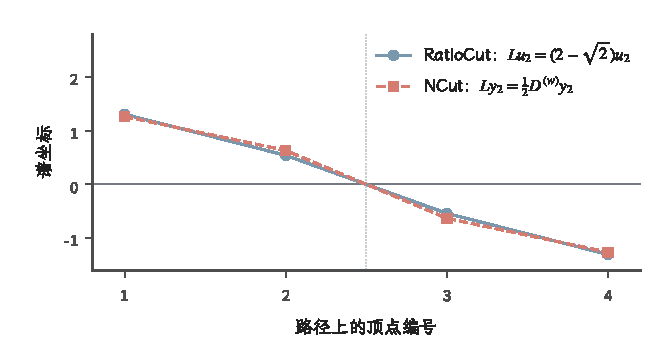
\includegraphics[width=\linewidth]{figures/math-preparation/reader-revision-graph/spectral-coordinates.pdf}
  \caption{单位边权路径\(1-2-3-4\)的两个精确谱方向。蓝实线为组合拉普拉斯的第二特征向量，红虚线为度加权广义特征向量；点形同时区分两者。为比较形状，图中两向量均按欧氏范数\(2\)缩放，此显示约定不改变各自的特征方程，也不替代NCut推导中的度加权范数。横轴只有四个顶点，连线仅引导阅读，竖虚线标出零阈值切分的位置。}
  \label{fig:graph-theory-spectral-coordinates}
\end{figure}

松弛向量不是离散分割本身。按符号或阈值切分会产生一个可行割，其目标值应回到原离散
目标计算。谱间隙小还意味着特征向量容易受扰动旋转；重复特征值时，稳定对象是特征子空间，
不是某个算法任意选出的单一基向量。

\subsection{图扩散与谱滤波}

平滑坐标描述一个静态信号，扩散则描述如何逐步减小相邻顶点的差异。
令每个顶点按邻居与自身的差值调整，即\(f_i'(t)=\sum_jw_{i,j}(f_j(t)-f_i(t))\)：
邻居较高就抬高本点，邻居较低就降低本点。把这些方程合在一起，正好得到负拉普拉斯作用。

连续时间图扩散定义为
\begin{equation}
  \frac{\mathrm{d}\bm{f}(t)}{\mathrm{d}t}
  =-\bm{L}\bm{f}(t),
  \qquad
  \bm{f}(0)=\bm{f}_0.
  \label{eq:graph-theory-heat-equation}
\end{equation}
第~\ref{chap:matrix-analysis}章的矩阵指数给出
\[
  \bm{f}(t)=\exp(-t\bm{L})\bm{f}_0
  =\sum_{k=1}^{n}e^{-t\lambda_k}
  \langle\bm{u}_k,\bm{f}_0\rangle\bm{u}_k.
\]
特征值大的模式衰减更快，零特征值对应的分量保持不变。正权支撑图连通时，
\(\bm{f}(t)\)趋向初始信号的常量投影；支撑图不连通时，每个支撑连通分量分别趋向
自己的平均。

总和保持来自\(\bm{1}^{\top}\bm{L}=\bm{0}^{\top}\)：
\[
  \frac{\mathrm{d}}{\mathrm{d}t}
  \bm{1}^{\top}\bm{f}(t)=0.
\]
平方范数与Dirichlet能量是两个不同的量。平方范数的导数恰好是负的Dirichlet能量：
\[
  \frac{\mathrm{d}}{\mathrm{d}t}
  \frac12\lVert\bm{f}(t)\rVert_2^2
  =
  -\bm{f}(t)^{\top}\bm{L}\bm{f}(t)
  \leq0.
\]
Dirichlet能量本身也下降，但对应的导数多出一个拉普拉斯：
\[
  \frac{\mathrm{d}}{\mathrm{d}t}
  \left[\bm{f}(t)^{\top}\bm{L}\bm{f}(t)\right]
  =
  -2\bm{f}(t)^{\top}\bm{L}^2\bm{f}(t)
  =
  -2\lVert\bm{L}\bm{f}(t)\rVert_2^2
  \leq0.
\]
第一个等式说明非平滑分量消耗平方范数，第二个等式直接说明边上平方差总量不会增加。
扩散因此削弱顶点间差异，但不表示它保留任务所需的类别边界。扩散时间过长会把同一
正权支撑连通分量内所有差异抹平。

在贯穿图上令每条边权为\(1\)，取\(\bm f_0=(1,0,0,0)^\top\)。其拉普拉斯特征值为\(0,2,4,4\)，因此不同频率的保留比例分别为\(1,e^{-2t},e^{-4t}\)。图~\ref{fig:graph-diffusion-spectrum}显示初始集中在顶点\(1\)的信号逐步分散；由于图连通且总和为\(1\)，极限为各顶点上的\(1/4\)，而不是信号全部消失。两个相同的特征值\(4\)对应不同特征向量，它们只是使用相同的衰减系数。

\begin{figure*}[htbp]
  \centering
  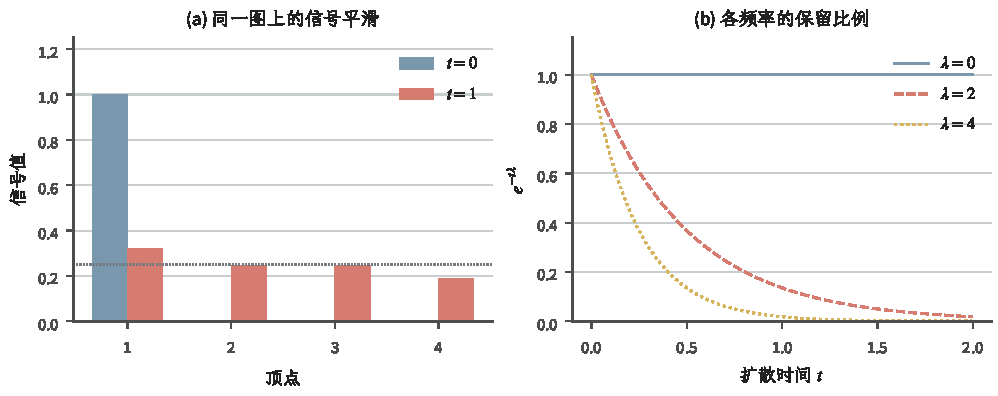
\includegraphics[width=\linewidth]{figures/math-preparation/probability-discrete/graph-diffusion-spectrum.pdf}
  \caption{贯穿四顶点图的解析式扩散。左图比较\(\bm f(0)=(1,0,0,0)^\top\)与\(\bm f(1)=e^{-\bm L}\bm f(0)\)，灰虚线为最终均值\(1/4\)；右图绘制三个不同特征值\(0,2,4\)的保留比例，特征值\(4\)实际具有重数\(2\)。柱与曲线由该图的拉普拉斯直接计算，不是仿真实验的均值或误差条。}
  \label{fig:graph-diffusion-spectrum}
\end{figure*}

\subsection{离散Dirichlet能量与连续极限}

式~\eqref{eq:graph-theory-dirichlet-energy}是第
~\ref{chap:differential-geometry-and-symmetry}章连续Dirichlet能量
\[
  \int_{\mathcal{M}}
  \lVert\operatorname{grad}f\rVert_g^2\,\mathrm{d}V_g
\]
的离散对应：连续梯度衡量无穷小方向的变化，图边差分只比较被连接的样本对。两者形式
相似，却不能只靠形式宣布收敛。

若图来自点云，邻域半径决定哪些局部方向被采样，核权重决定不同距离的贡献，归一化决定
是否保留采样密度，边界又会改变极限条件。邻域过大可能跨越弯曲流形的不同折，过小则使
图断连。样本密度不均时，未校正的图拉普拉斯可能逼近带密度漂移的算子，而不是纯粹由
Riemann体积定义的Laplace--Beltrami算子。

因此，图谱只相对于已经选定的图和权重给出精确代数结论。它是否近似某个连续空间，
需要额外的采样、尺度与归一化条件；它是否保留预测语义，又需要任务证据。

\section{在重编号下保持表示并比较图结构}
\label{sec:graph-theory-structure-comparison}

图的顶点编号可以任意改变。一个结构表示既要避免把编号差异当成结构差异，又需要区分真正不同的图。这是两个要求：等变或不变性解决前者，局部细化的区分能力关系到后者。下面先检验拉普拉斯和滤波器的置换行为，再以多重集合细化展示局部表示的能力边界。

\subsection{顶点置换与等变性}

顶点级输出和整图级输出需要不同的编号行为。例如预测每个顶点的数值，重新编号后预测也应随顶点重排，
这称为等变；判断整张图是否连通，重新编号后答案应保持相同，这称为不变。
这两个术语的完整定义见定义~\ref{def:geometry-equivariant-map}与定义~\ref{def:geometry-invariant-map}；这里把它们用于有限置换。

顶点名称只是坐标标签。同一图经置换矩阵\(\bm{P}\)重编号后，
\[
  \bm{W}'=\bm{P}\bm{W}\bm{P}^{\top},
  \qquad
  \bm{D}^{(w)\prime}=\bm{P}\bm{D}^{(w)}\bm{P}^{\top},
  \qquad
  \bm{L}'=\bm{P}\bm{L}\bm{P}^{\top}.
  \label{eq:graph-theory-laplacian-relabel}
\]
若顶点信号也重编号为\(\bm{f}'=\bm{P}\bm{f}\)，则
\[
  \bm{L}'\bm{f}'=\bm{P}\bm{L}\bm{f}.
\]
图拉普拉斯作用因此对顶点置换等变：输入顶点怎样重排，输出按同样方式重排。

更一般地，图滤波器若为多项式
\begin{equation}
  h(\bm{L})=\sum_{k=0}^{K}a_k\bm{L}^k,
  \label{eq:graph-theory-polynomial-filter}
\end{equation}
则
\[
  h(\bm{L}')\bm{f}'
  =\sum_{k=0}^{K}a_k(\bm{P}\bm{L}\bm{P}^{\top})^k\bm{P}\bm{f}
  =\bm{P}h(\bm{L})\bm{f},
\]
因为\(\bm{P}^{\top}\bm{P}=\bm{I}\)。若再对顶点输出作求和等对称汇总，可以得到置换
不变的图级表示。等变性只保证结果不依赖任意编号，不保证不同非同构图一定得到不同表示。

两张无向图\(\mathcal G=(V,E)\)与\(\mathcal G'=(V',E')\)若存在顶点双射\(\rho:V\to V'\)，使
\[
  \{i,j\}\in E\quad\Longleftrightarrow\quad\{\rho(i),\rho(j)\}\in E',
\]
就称为\term{同构}（isomorphic）。它表示忽略顶点名称后，连接关系完全相同；对有向图要保持有序弧的方向，
若比较加权图，还要保持对应边的权重。
无权图或所有结构边权均非零的加权图，可以等价地用置换矩阵条件
\(\bm A'=\bm P\bm A\bm P^\top\)判断同构。若允许零权结构边，则还必须核对边集或邻接掩码：
两顶点空图与含一条零权边的图都可以有\(\bm A=\bm0\)，却有不同连接结构。
即便矩阵足以确定结构，也不能用一般特征分解替代置换判据：同谱图可能不同构，重复特征值下特征向量基也不唯一。

\subsection{多重集合细化与局部结构}

与编号无关还不够：把每张图都映成同一个常数也满足不变性，却没有区分结构的能力。
一个更有信息的做法是反复比较每个顶点看到的邻域，把局部形态不同的顶点逐渐区分开。
为了不依赖邻居的排列顺序，同时保留某类邻居有多少个，需要使用多重集合。

邻居没有天然顺序，所以一个顶点的局部结构应通过邻居标记的
\term{多重集合}（multiset）表示。多重集合既记录元素种类，也记录每种元素出现次数；
\(\{a,a,b\}\)与\(\{a,b\}\)不同，但不区分排列次序。

\begin{definition}[一维邻域标记细化]
\label{def:graph-theory-wl-refinement}
一维Weisfeiler--Leman细化（1-dimensional Weisfeiler--Leman refinement,
1-WL）从初始标记\(c_i^{(0)}\)出发，反复令
\begin{equation}
  c_i^{(t+1)}=\operatorname{HASH}\left(
    c_i^{(t)},
    \left\{\!\left\{
      c_j^{(t)}:j\in N(i)
    \right\}\!\right\}
  \right),
  \label{eq:graph-theory-wl-refinement}
\end{equation}
其中\(\operatorname{HASH}\)对不同输入对给出不同新标记。每轮都把顶点自身旧标记与
邻居标记多重集组合。
\end{definition}

\(\operatorname{HASH}\)在这里是无碰撞编码的数学约定，不能直接假定一个普通有限哈希函数也绝不碰撞。
比较两张图时须使用一致的初始标记规则和同一编码对应；任意各自起名会使标记名称不可比较。
由于输入只包含自身标记与无序邻居计数，同构重编号只会同步重排标记，不改变各标记的出现次数。

这个过程会在有限步后稳定。令\(\mathcal{P}^{(t)}\)表示按
\(c_i^{(t)}\)相等关系得到的顶点分区。由于更新输入包含顶点自身旧标记，旧标记不同的
两个顶点下一轮仍不可能获得相同标记，所以
\(\mathcal{P}^{(t+1)}\)只能细分\(\mathcal{P}^{(t)}\)，不能合并其中的块。若分区
尚未稳定，块数至少增加\(1\)；而\(n\)个顶点至多分成\(n\)个非空块。因此从任意初始
分区出发，严格细分至多发生\(n-1\)次。某轮分区不再改变后，下一轮每个块中的顶点仍有
相同的自身标记和邻居标记计数，后续分区也保持不变。这里的“稳定”指等价类不再细分，
哈希实现仍可为这些类换用新的符号名称。

细化稳定不表示已经解决图同构。若所有顶点初始同标记，六顶点环\(C_6\)与两个互不相连
的三角形都让每个顶点始终看到两个同标记邻居；1-WL无法区分二者，尽管一张图连通、另一张
不连通。若把任意顶点编号当作固定初始特征，结果就会依赖编号，不能作为这个无标记图比较问题的无条件补救。
额外顶点属性若随置换同步移动，算法仍可等变，但输入已改成带属性图；那是另一个比较设定。

\begin{figure}[htbp]
  \centering
  \begingroup
% Local styles; callers keep this input inside a group.
\tikzset{
  reader vertex/.style={circle,draw=FigureStroke,fill=white,line width=1pt,
    minimum size=7mm,inner sep=0pt,font=\figurefont\footnotesize,text=FigureInk},
  reader factor/.style={rectangle,draw=FigureStroke,fill=FigureYellowFill,
    line width=1pt,minimum size=8mm,inner sep=2pt,font=\figurefont\footnotesize},
  reader edge/.style={draw=FigureStroke,line width=1.1pt},
  reader arrow/.style={reader edge,-{Stealth[length=2.2mm,width=1.4mm]}},
  reader label/.style={font=\figurefont\footnotesize,text=FigureInk},
  reader note/.style={reader label,fill=white,inner sep=1pt},
  reader highlight/.style={draw=FigureYellow,line width=1.1pt},
  reader auxiliary/.style={draw=FigureMuted,line width=0.6pt,dashed}
}

\begin{tikzpicture}[text=FigureInk]
  \node[reader label] at (0,1.7) {(a) 六顶点环 \(C_6\)};
  \foreach \i in {1,...,6}
    \node[reader vertex,fill=FigureYellowFill] (a\i) at ({90-60*(\i-1)}:1.1) {};
  \foreach \i/\j in {1/2,2/3,3/4,4/5,5/6,6/1}
    \draw[reader edge] (a\i)--(a\j);
  \node[reader label] at (5.2,1.7) {(b) 两个不相交三角形};
  \foreach \x/\prefix in {3.8/b,6.6/c}
  {
    \node[reader vertex,fill=FigureYellowFill] (\prefix1) at (\x,0.9) {};
    \node[reader vertex,fill=FigureYellowFill] (\prefix2) at (\x-0.75,-0.6) {};
    \node[reader vertex,fill=FigureYellowFill] (\prefix3) at (\x+0.75,-0.6) {};
    \draw[reader edge] (\prefix1)--(\prefix2)--(\prefix3)--(\prefix1);
  }
  \node[reader label] at (0,-1.85) {每个顶点：2个同标记邻居};
  \node[reader label] at (5.2,-1.85) {每个顶点：2个同标记邻居};
\end{tikzpicture}
\endgroup

  \caption{相同局部计数不保证相同整体结构。所有顶点从同一标记开始，每轮都看见两个同标记邻居，因此两张六顶点图的1-WL标记计数始终相同。左图只有一个连通分量，右图有两个；这证明该局部细化不能在这个例子中识别连通性的差异，而不是说连通性本身难以计算。浅黄填充只表示同标记，圆内不放唯一编号，以免改变例子的输入。}
  \label{fig:graph-theory-wl-local-ambiguity}
\end{figure}

1-WL提供的是局部组合表达的参照。使用共享顶点更新和对称邻域聚合的具体图网络能否达到、
低于或超过该区分能力，要在模型正文中根据聚合函数、初始特征和读出方式证明。本章只建立
多重集合、置换作用和细化过程，不把结构等变性升级成学习能力或泛化保证。

\section{本章小结}
\label{sec:graph-theory-summary}

图的第一个作用是保留关系的结构，表示方式必须与查询相匹配。普通边、带方向的弧和高阶因子的作用域保留的信息不同，不能把一张关系图自动解释成概率或因果模型。
条件独立查询还会随条件集合改变：祖先道德化为每个DAG查询提供无向判据，但只有满足完美性与弦图条件时，才存在保存全部分离答案的固定等价表示。

图的第二个作用是组织计算。先明确要求总权重、边缘量还是最优配置，再选择组合与汇总运算，消元才有确定含义。
分配律保证汇总内部变量时保留原查询，分隔集和树分解则限制中间表的依赖范围。
贯穿例先处理顶点\(1,4\)只需宽度\(2\)，先处理顶点\(2\)却产生填充边\(\{1,4\}\)和宽度\(3\)。
弦图刻画无需补边的完美消元序，树宽衡量能达到的最小袋宽度；两者都不取代对取值域、因子成本和查询运算次序的检查。
针对特殊目标，还可以利用更强结构：非负边长支持Dijkstra的贪心确定，割性质支持最小生成树，容量与守恒使最大流和最小割构成同值证书，二部匹配借助整数流完成配对，二值次模能量则能写成非负割容量。
这些保证各自服务于不同目标，不能仅凭图的外形选择算法。精确结构不足时，可行解与松弛下界共同说明当前答案离最优至多有多远。

图的第三个作用是构造信号与结构表示。拉普拉斯能量度量沿边的变化，谱松弛把离散分割转成实数坐标，扩散按特征值衰减非平滑成分。
RatioCut按顶点数平衡，NCut按加权体积平衡，所以两者的特征方程不同；连续极限还依赖图构造、采样密度、尺度与边界。
置换等变性保证顶点级输出随重编号同步变化，不变性保证整图输出不受编号影响，二者都不保证表示足够丰富。
六环与两个三角形的1-WL反例表明：正确的对称性和相同局部计数仍可能遗漏整体差异。

读者据此可以把一个图问题分成具体判断：表示是否保留所需关系，查询采用何种运算，结构能否缩小计算规模，以及输出是否有相应的正确性或误差证书。
第~\ref{chap:signal-analysis}章转向有顺序的信号，比较规则序列频率与这里的图频率，再把线性递推展开成随时间组织的状态核。
